\section{Architectural Design}
\subsection{Overview: high-level components and interactions}
\begin{figure}[H]
    \begin{center}
        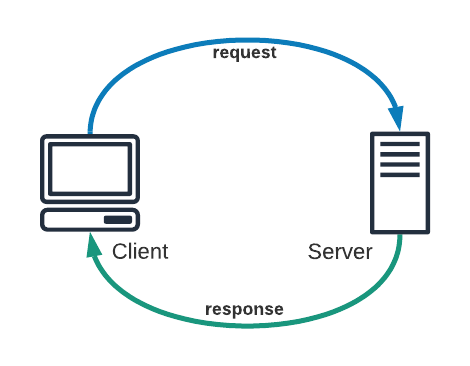
\includegraphics[width=\textwidth/2]{img/Client-Server.png}
        \caption{Client-Server paradigm}\label{client_server_par}
    \end{center}
\end{figure}

As figure \ref{client_server_par} represents, the system is a distributed application which follows the common known client-server paradigm.

In particular, there are two different types of client-server interactions, because the product has 2 modules that need to fulfill different goals for different actors. 

Since Module 1 will feature a mobile application, that will contain an internal database in order to make it less dependent from the server. This aspect makes it a more of a thick client.

Module 2, on the other hand, will feature a \textit{Web Application}, which is by definition a thin client, because of its total dependency from the server.
This type of client does not contain the application business logic, but only the presentation layer.

In both cases the server is \textit{fat} and contains all the data management and business logic.

In this section the architecture will be described in an easy way, justifying all the choices for adopted patterns.

\begin{figure}[H]
    \begin{center}
        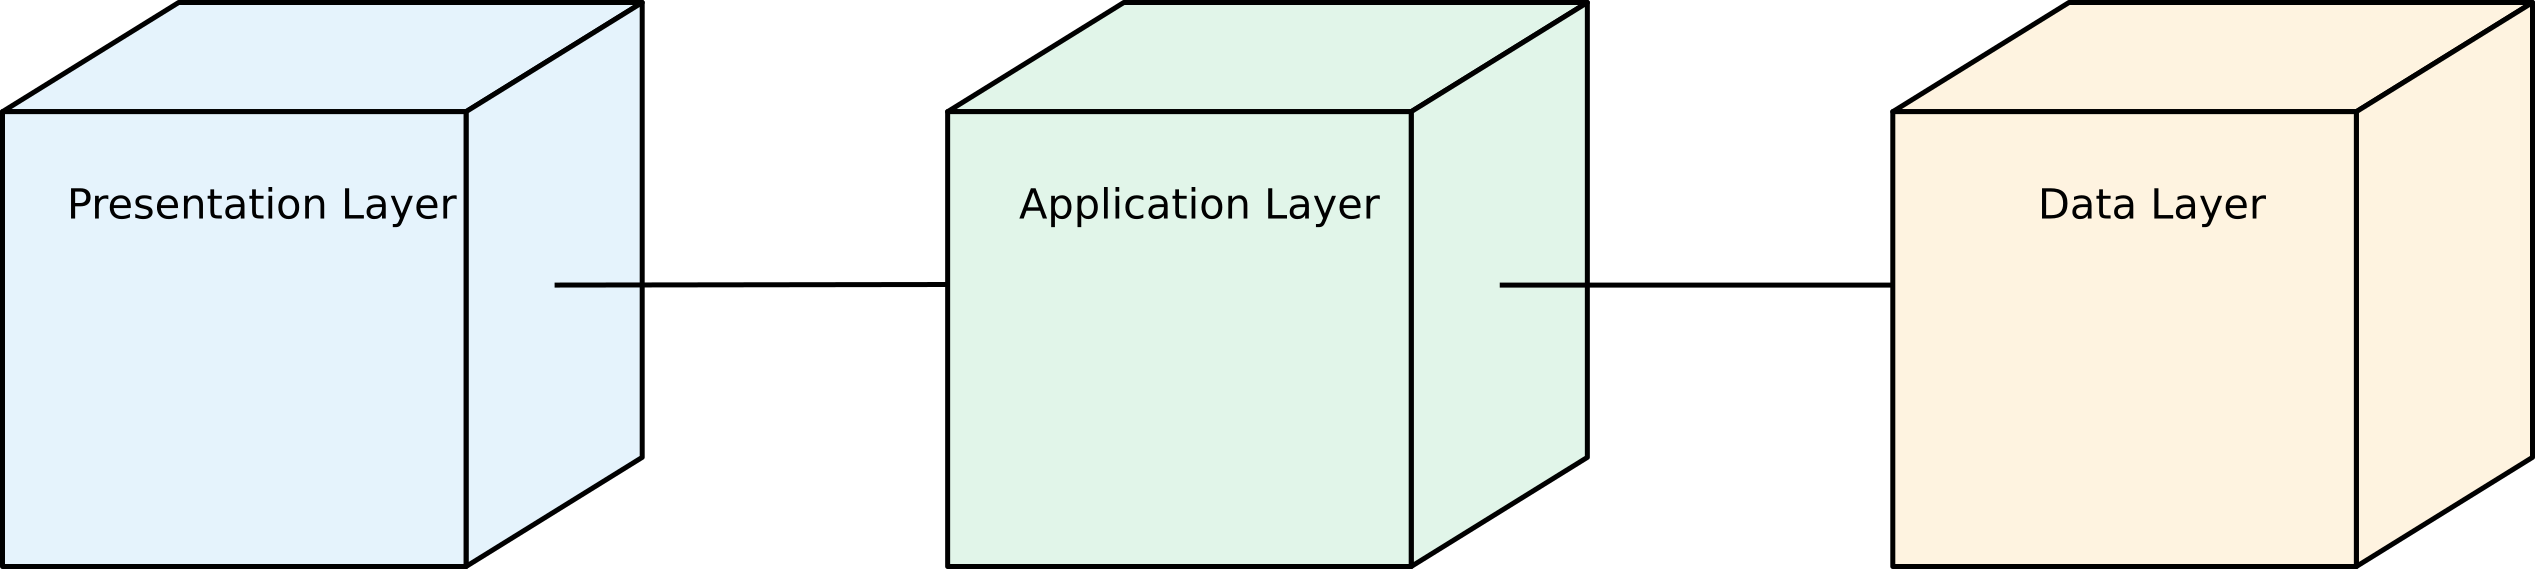
\includegraphics[width=\textwidth]{img/3-tier.png}
        \caption{Three layers application}\label{three_tier_desc}
    \end{center}
\end{figure}

In figure \ref{three_tier_desc} the three S2B layers are shown, which respectively are:
\begin{itemize}
    \item \textbf{Presentation Layer:} it manages the presentation logic and, consequently, all the interactions with the end user. This is also called \textit{rendering layer}.
    \item \textbf{Application (Logic) Layer:} it manages the business functions that the S2B must provide.
    \item \textbf{Data Layer:} it manages the safe storage and the relative access to data.
\end{itemize}

As shown in the high level representation of figure \ref{architecture_overview} the S2B is divided into three layers that are physically separated by installing them on different tiers. A tier is a physical (or a set of) machine, each of them with its own computational power.

The application described in this document is composed by four tiers.

\begin{figure}[H]
    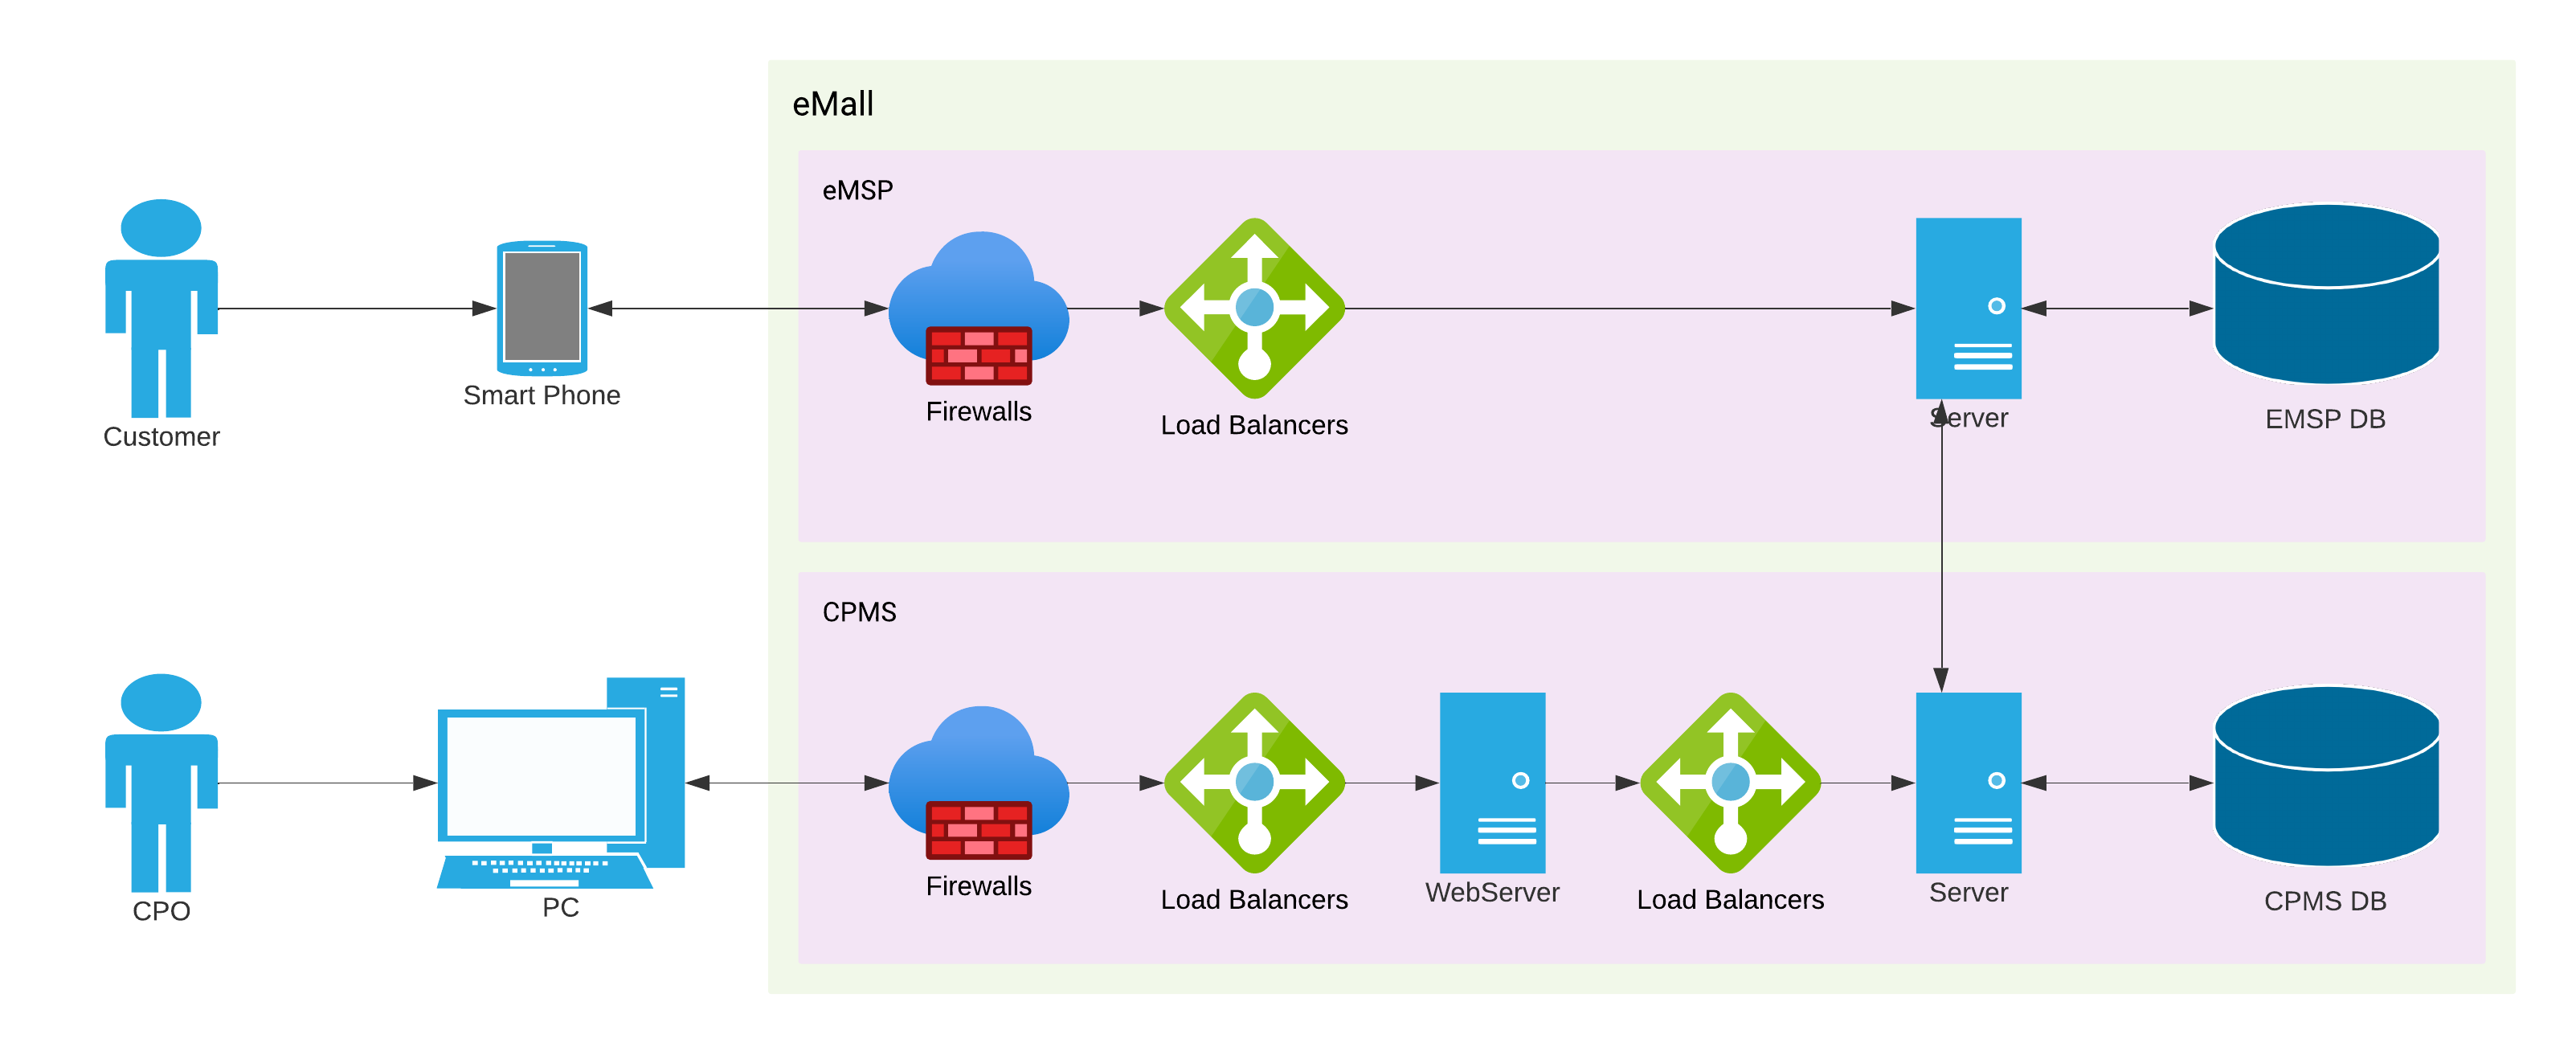
\includegraphics[width=\textwidth]{img/ArchitectureOverview.png}
    \caption{Architecture of the application}\label{architecture_overview}
\end{figure}    


\subsection{Component view}

In this section there is an high-level analysis of the main components and their subcomponents. Main interfaces interactions between components are also provided.

\begin{figure}[H]
    \begin{center}
        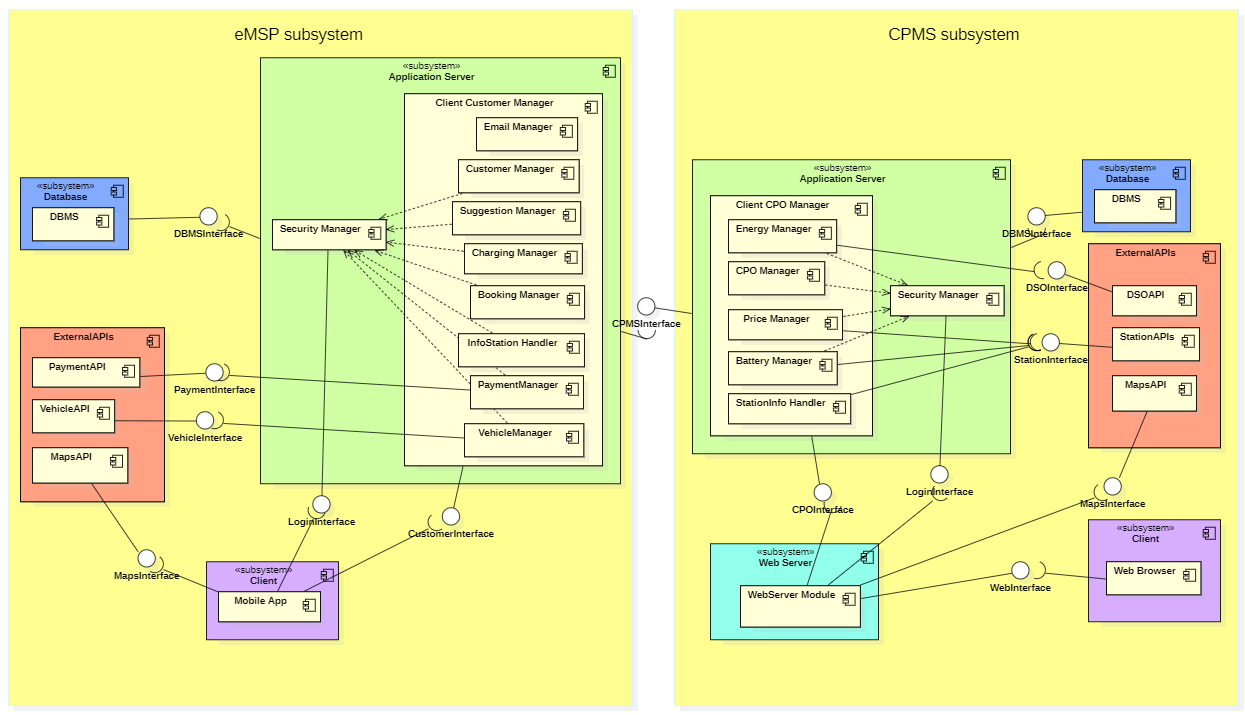
\includegraphics[width=\textwidth]{img/ComponentDiagram.PNG}
        \caption{Component Diagram}\label{component_diagram}
    \end{center}
\end{figure}




eMSP's components:
\begin{itemize}
    \item \textbf{Client Customer Manager}\\This module handles all the requests made by the client. At the beginning, when the client is not logged in, the module offers (through the customer manager) a LoginInterface which permits to execute a sign up or sign in operation. Once the client has logged in, the module shows only the CustomerInterface which the customer will exploit.
    \item \textbf{Email Manager}\\This component handles the email notifications, such as the sign up and forgot password ones.
    \item \textbf{Customer Manager}\\This module contains all the features in order to manage the customer side. In fact, it includes the log in and sign up manager.
    
    \item \textbf{Suggestion Manager}\\This module manages the push notifications. Based on the information aquired thanks to the Vehicle Manager, it creates suggested bookings and shows all the details about them. It allows also to confirm a suggested booking on the application.
    \item \textbf{Charging Manager}\\ This module manages the charging process operations, such as the socket unlocking. It also shows the remaining time to end a charge and the charging state (in charge/ finished).
    \item \textbf{Booking Manager}\\This component manages the booking process. It aims to handle the sockets' booking and shows the details of the different bookings.
    \item \textbf{InfoStation Handler}\\This component handles the information about the charging stations. So it shows information about sockets types and related prices and special offers, sockets availabity and specifications about the charging stations.
    \item \textbf{Payment Manager}\\This component's aim is to handle the customer payment. It uses a PaymentAPI in order to process the task.
    \item \textbf{Vehicle Manager}\\This component's aim is to get the customer's vehicle information, such as the position, the battery percentage and the calendar.
    \item \textbf{Security Manager}\\Finally, this components handles all the security issues of the S2B. In fact, its aim is to authenticate and authorize requests, relying on the token provided from the client (since it should be a REST application). If a request is not authenticated, it takes the user to a login page; otherwise it simply replies with an unauthorized state message.
\end{itemize}

CPMS's components:
\begin{itemize}
    \item \textbf{Client CPO Manager}\\This module handles all the requests made by the client. At the beginning, when the client is not logged in, the module offers (through the CPO manager) a LoginInterface which permits to execute a sign in operation. Once the client has logged in, the module shows only the CPOInterface which the CPO will exploit.
    \item \textbf{Energy Manager}\\This module's aim is to handle the energy options.
    It also allows to select a DSO and aquire energy from it. On the other hand allows to set some operations such as the auto-mode.
    \item \textbf{CPO Manager}\\This module contains all the features in order to manage the user side. It includes the log in manager.
    \item \textbf{Price Manager}\\This module in needed to set special offers on socket's types in selected charging stations. Moreover it is used to set socket prices.
   
    \item \textbf{Battery Manager}\\This component manages the battery in the charging stations. It handles the battery policy change.
    \item \textbf{StationInfo Handler}\\This component handles the information about the charging stations. So it shows information about sockets types and related prices and special offers, sockets availabity and specifications about the charging stations.
 
    \item \textbf{Security Manager}\\Finally, this components handles all the security issues of the S2B. In fact, its aim is to authenticate and authorize requests, relying on the token provided from the client (since it should be a REST application). If a request is not authenticated, it takes the user to a login page; otherwise it simply replies with an unauthorized state message.
\end{itemize}

\subsection{Deployment view}

\begin{figure}[H]
    \begin{center}
        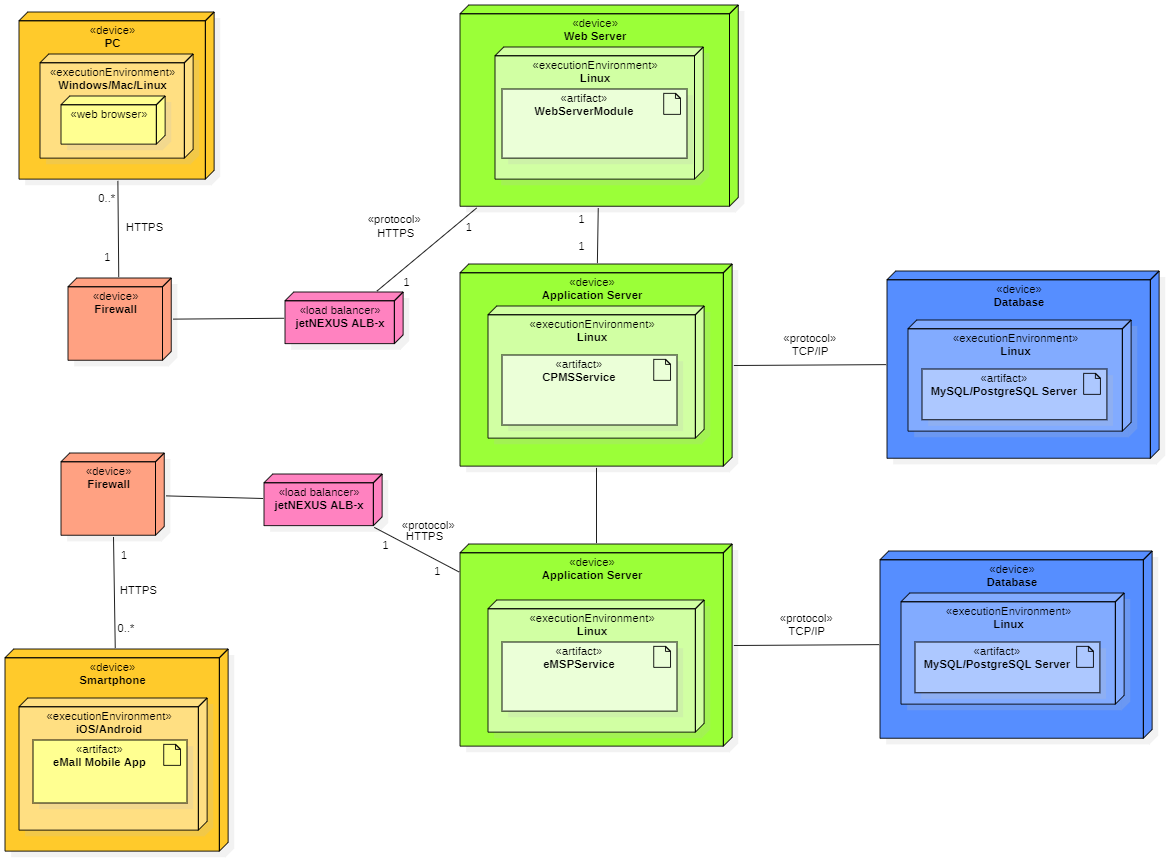
\includegraphics[width=\textwidth]{img/DeploymentDiagram.PNG}
        \caption{Deployment Diagram}\label{deployment_diagram}
    \end{center}
\end{figure}

The deployment diagram in figure\ref{deployment_diagram} shows the needed components for a correct system behavior and the protocols to communicate. As shown in the above image, firewalls and load balancers manage the data stream
from the devices to the servers. First of all, firewalls are in charge of filtering packets
received from the Internet. Then, the packets pass through the load balancer, where
the workload is distributed among the available resources to increase capacity and
reliability.
Each device has its own Operating System where the software runs.
The tiers in the image are the following:
\begin{itemize}
    \item \textbf{Tier 1:} it is the client machine, which can be a computer with a web browser (running, for example, on Windows 10 OS) or the downloadable mobile application (available on both Apple's store and Google's Store).
    \item \textbf{Tier 2:} it includes the replicated web servers, which do not execute any business logic, but simply receive requests from the client, route them to the application servers and serve an HTML file fo the client, which will build the page thanks to client-side scripting. They also append the styling logic of the page (CSS sheets, JS sheets, etc.).
    \item \textbf{Tier 3:} it contains the application servers, which run the core functionalities of the S2B. The whole application layer is mapped into this tier, which communicates to the client tier through APIs, which will be used from the web servers (in case of webapp) and the native application (in case of mobile app download). Furthermore, it communicates to the data tier through the DBMS gateway.
    \item \textbf{Tier 4:} it is composed by the DBMS servers. They store the data and execute actions on it, according to the instruction given by the application servers.
\end{itemize}
\subsection{Runtime view}
As stated previously, Module 1 (eMSP subsystem) is a mobile app while Module 2 (CPMS subsystem) is a web app. All the following diagrams represent the runtime view from the mobile app’s perspective, in order to increase readability, the web app’s perspective isn’t shown as it only differs from the other one by using the web server’s module before calling the Application Server.\\
Every interface uses the REST API through HTTP GET or/and POST calls.
\subsubsection{Signup Customer}
\begin{figure}[H]
    \begin{center}
        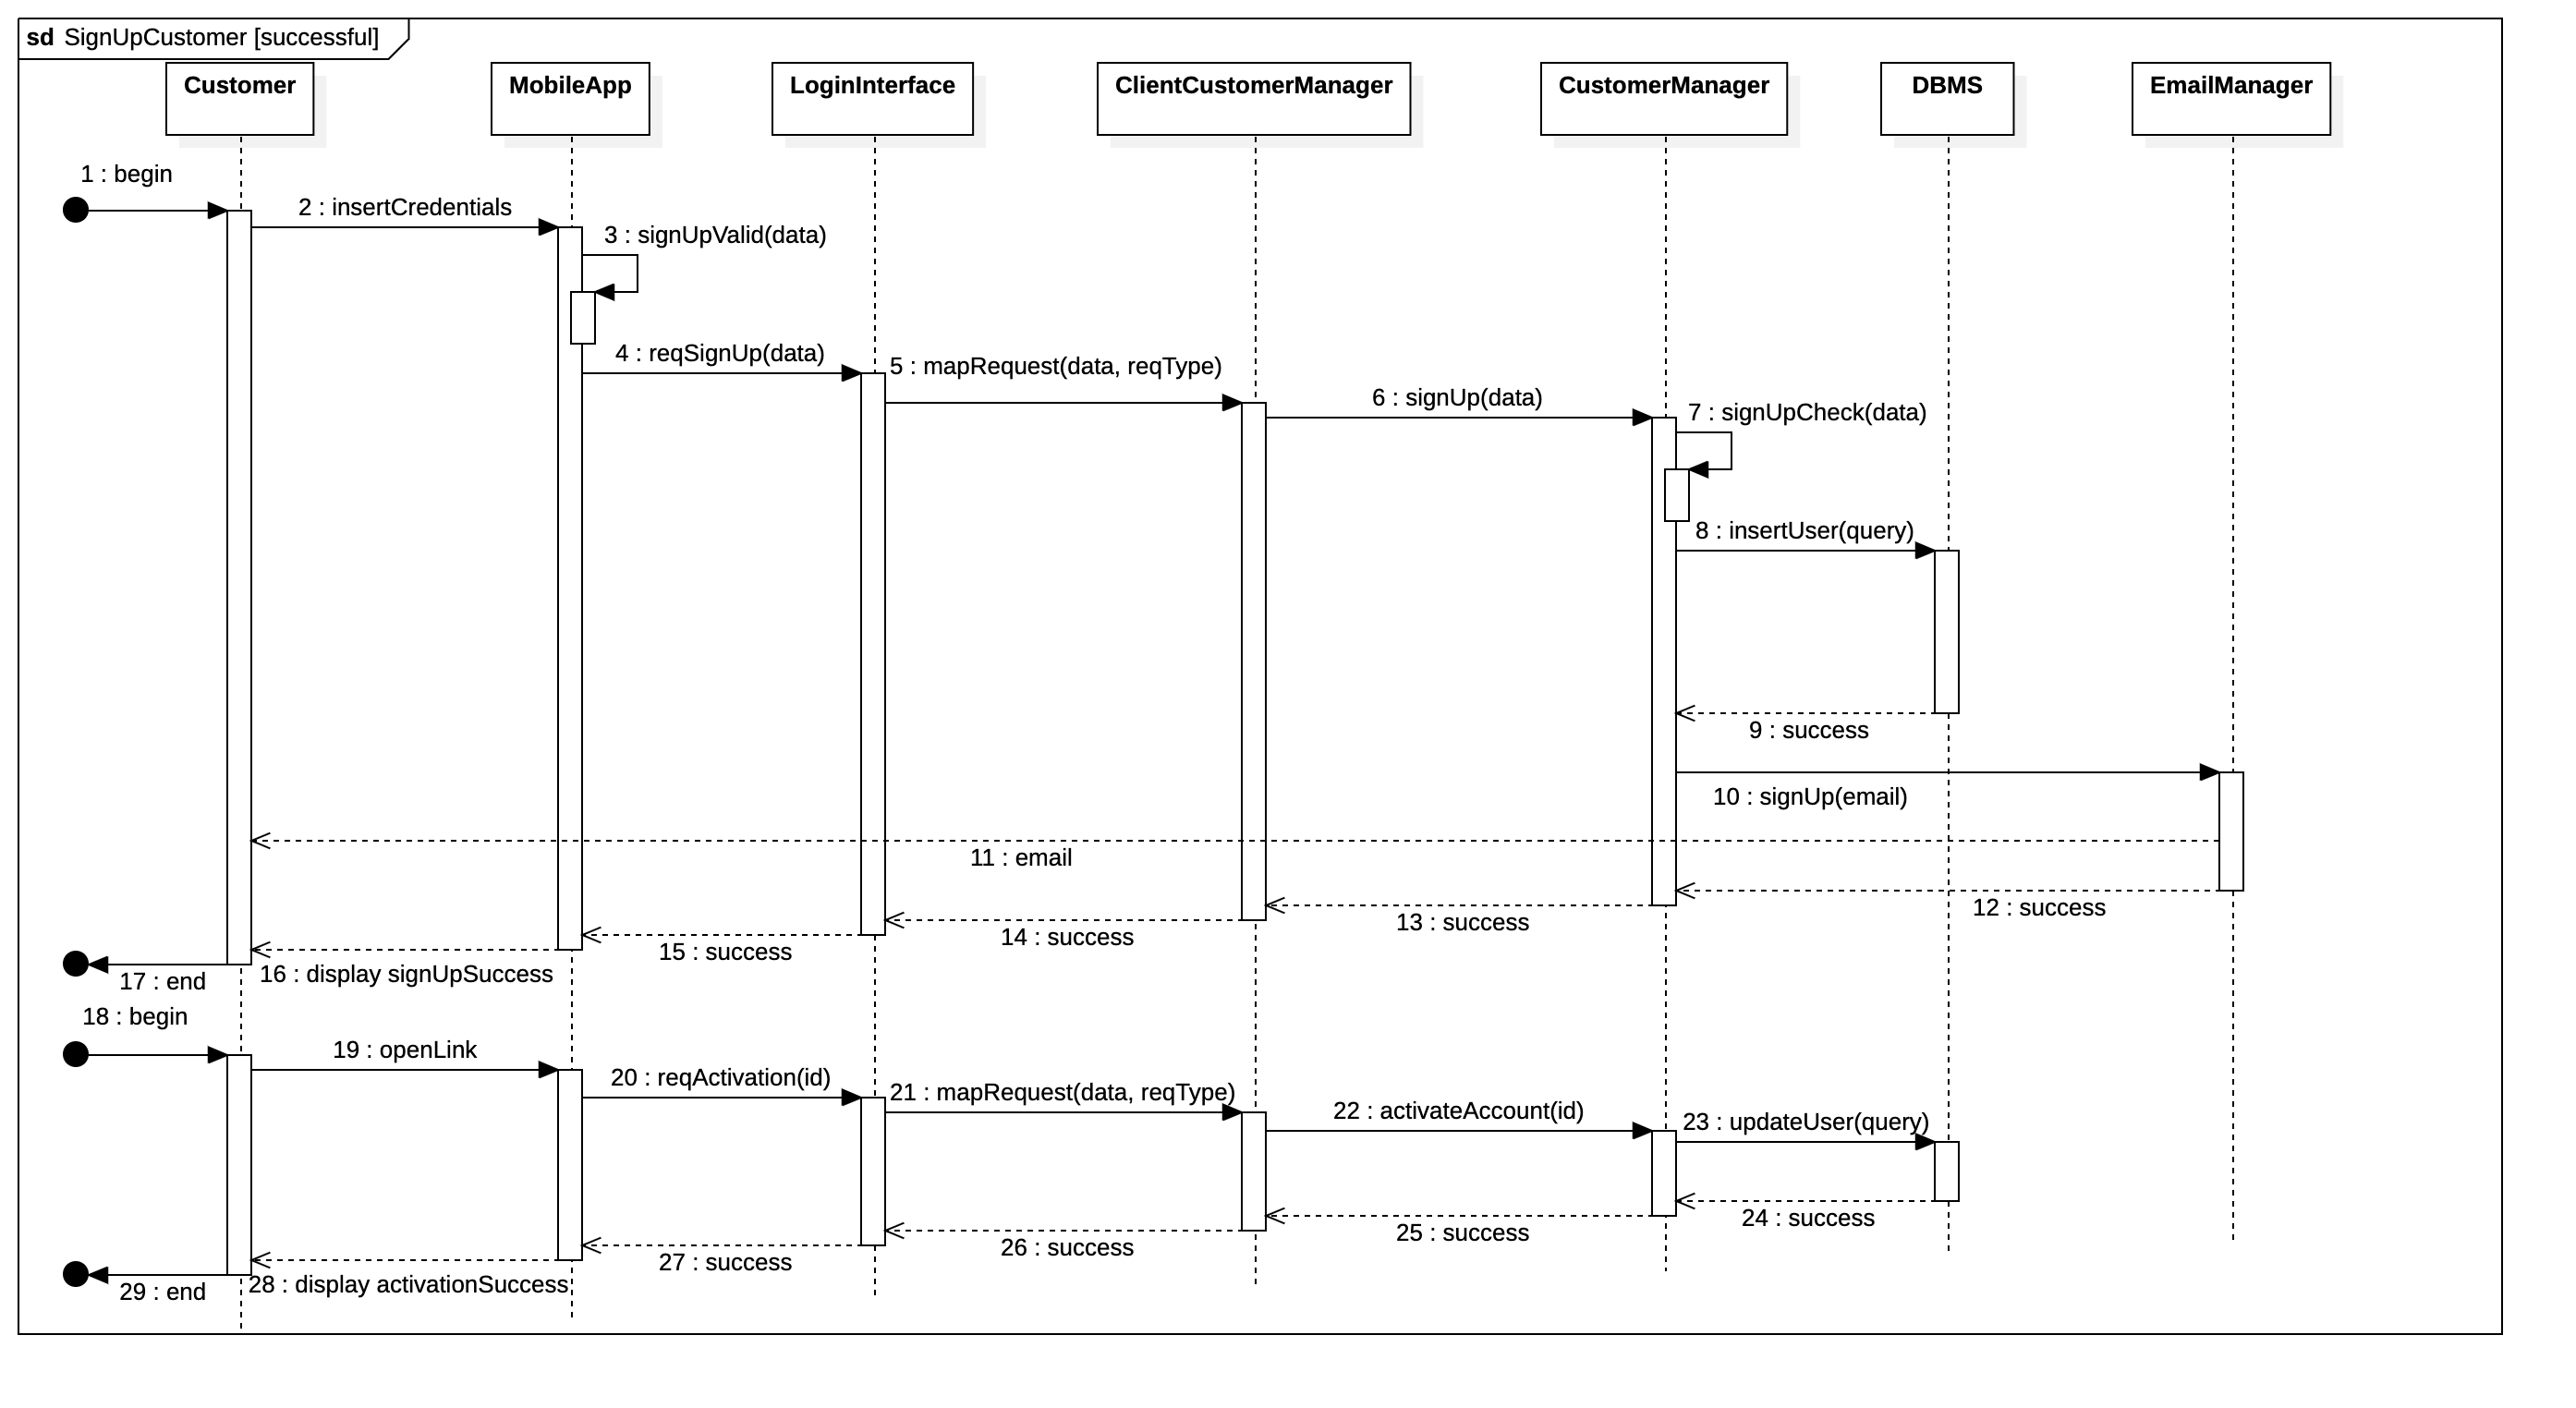
\includegraphics[width=\textwidth]{img/runtime/cust_signup_success}
        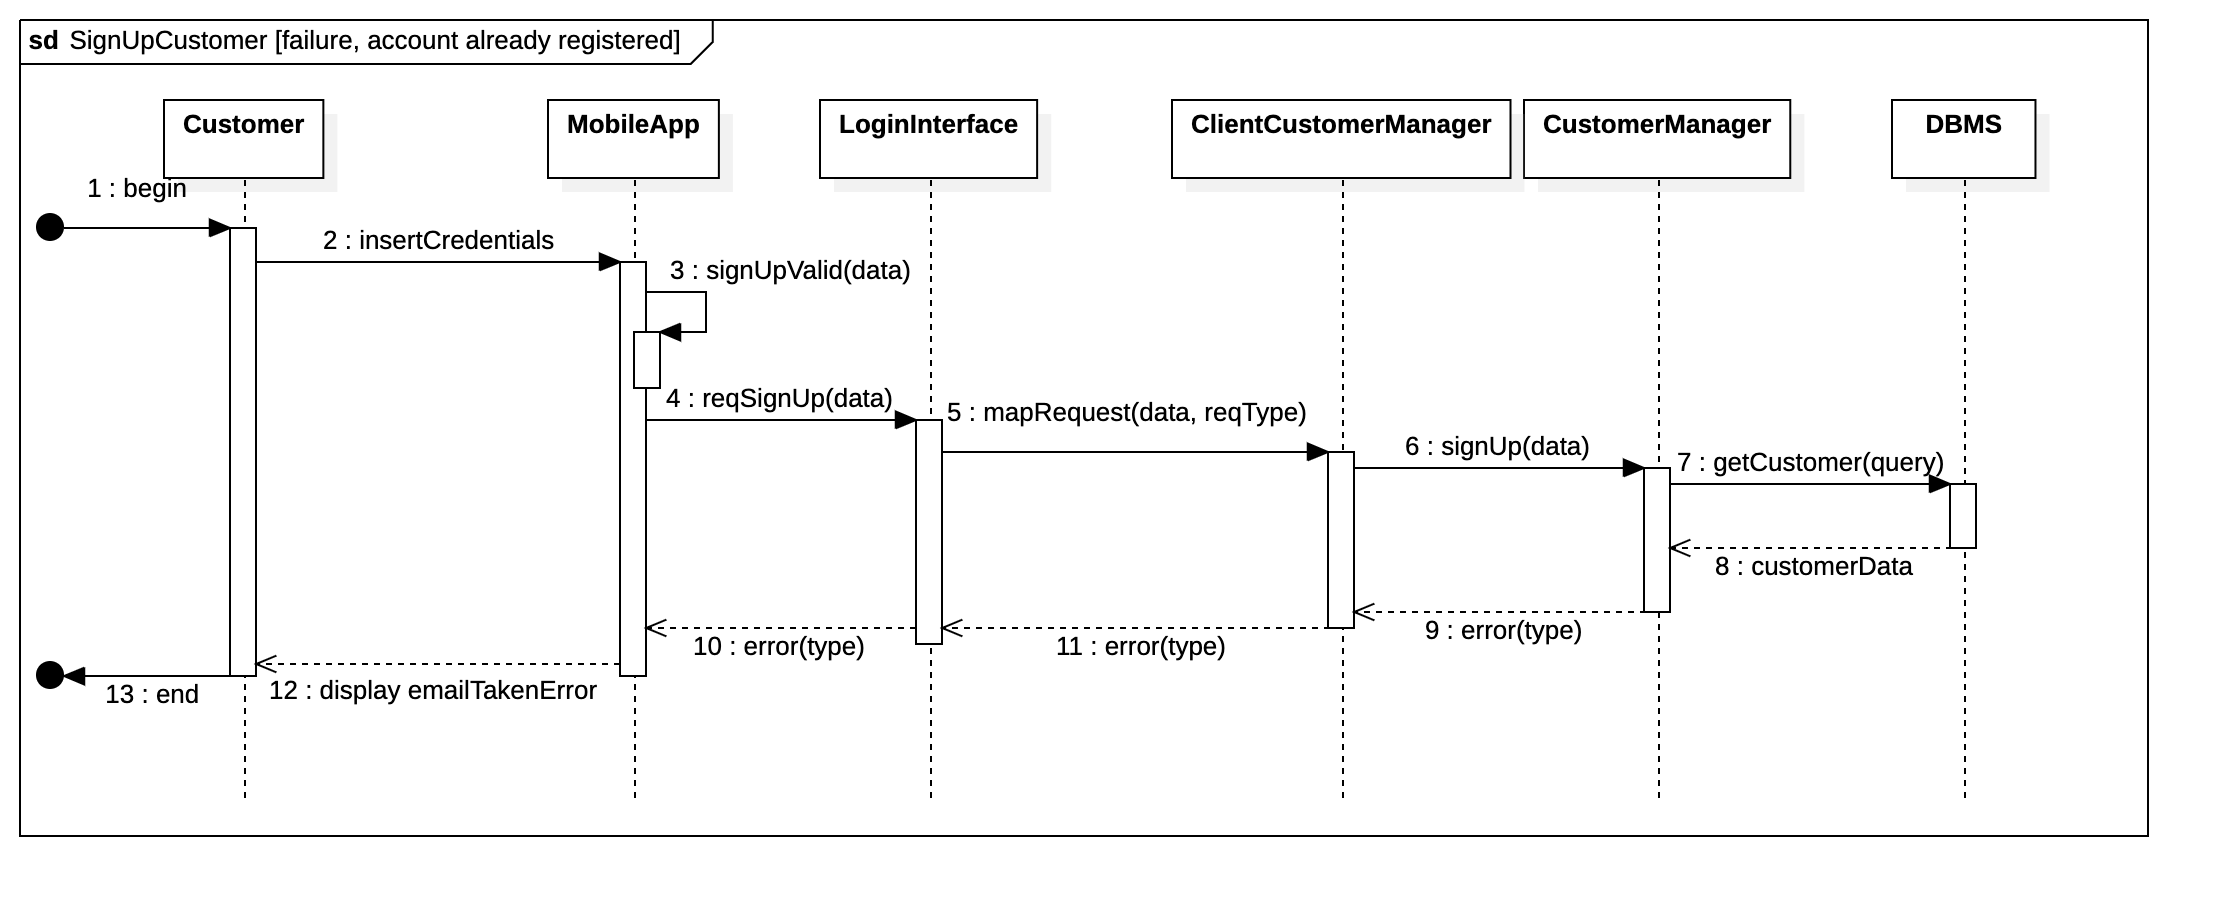
\includegraphics[width=\textwidth]{img/runtime/cust_signup_error}
    \end{center}
\end{figure}
The diagram above represents the process of signing up a Customer. There two possible situations:
\begin{itemize}
    \item Customer performs a correct registration process;
    \item Customer performs a wrong registration process (such as the account is already registered or the email in not valid).
\end{itemize}
The Customer begins by inserting his registration credentials in the app. Afterwards the app sends the request to the ClientCustomerManager through the LoginInterface, accessing later the CustomerManager.\\
The CustomerManager checks for the correctness of the received information and if correct it passes it ultimately to the DBMS. Then an email is sent to the Customer by the EmailManager. If the CustomerManager checks fail, the user is sent a specific error message related to his issue.
\subsubsection{Login Customer}\label{cust_login}
\begin{figure}[H]
    \begin{center}
        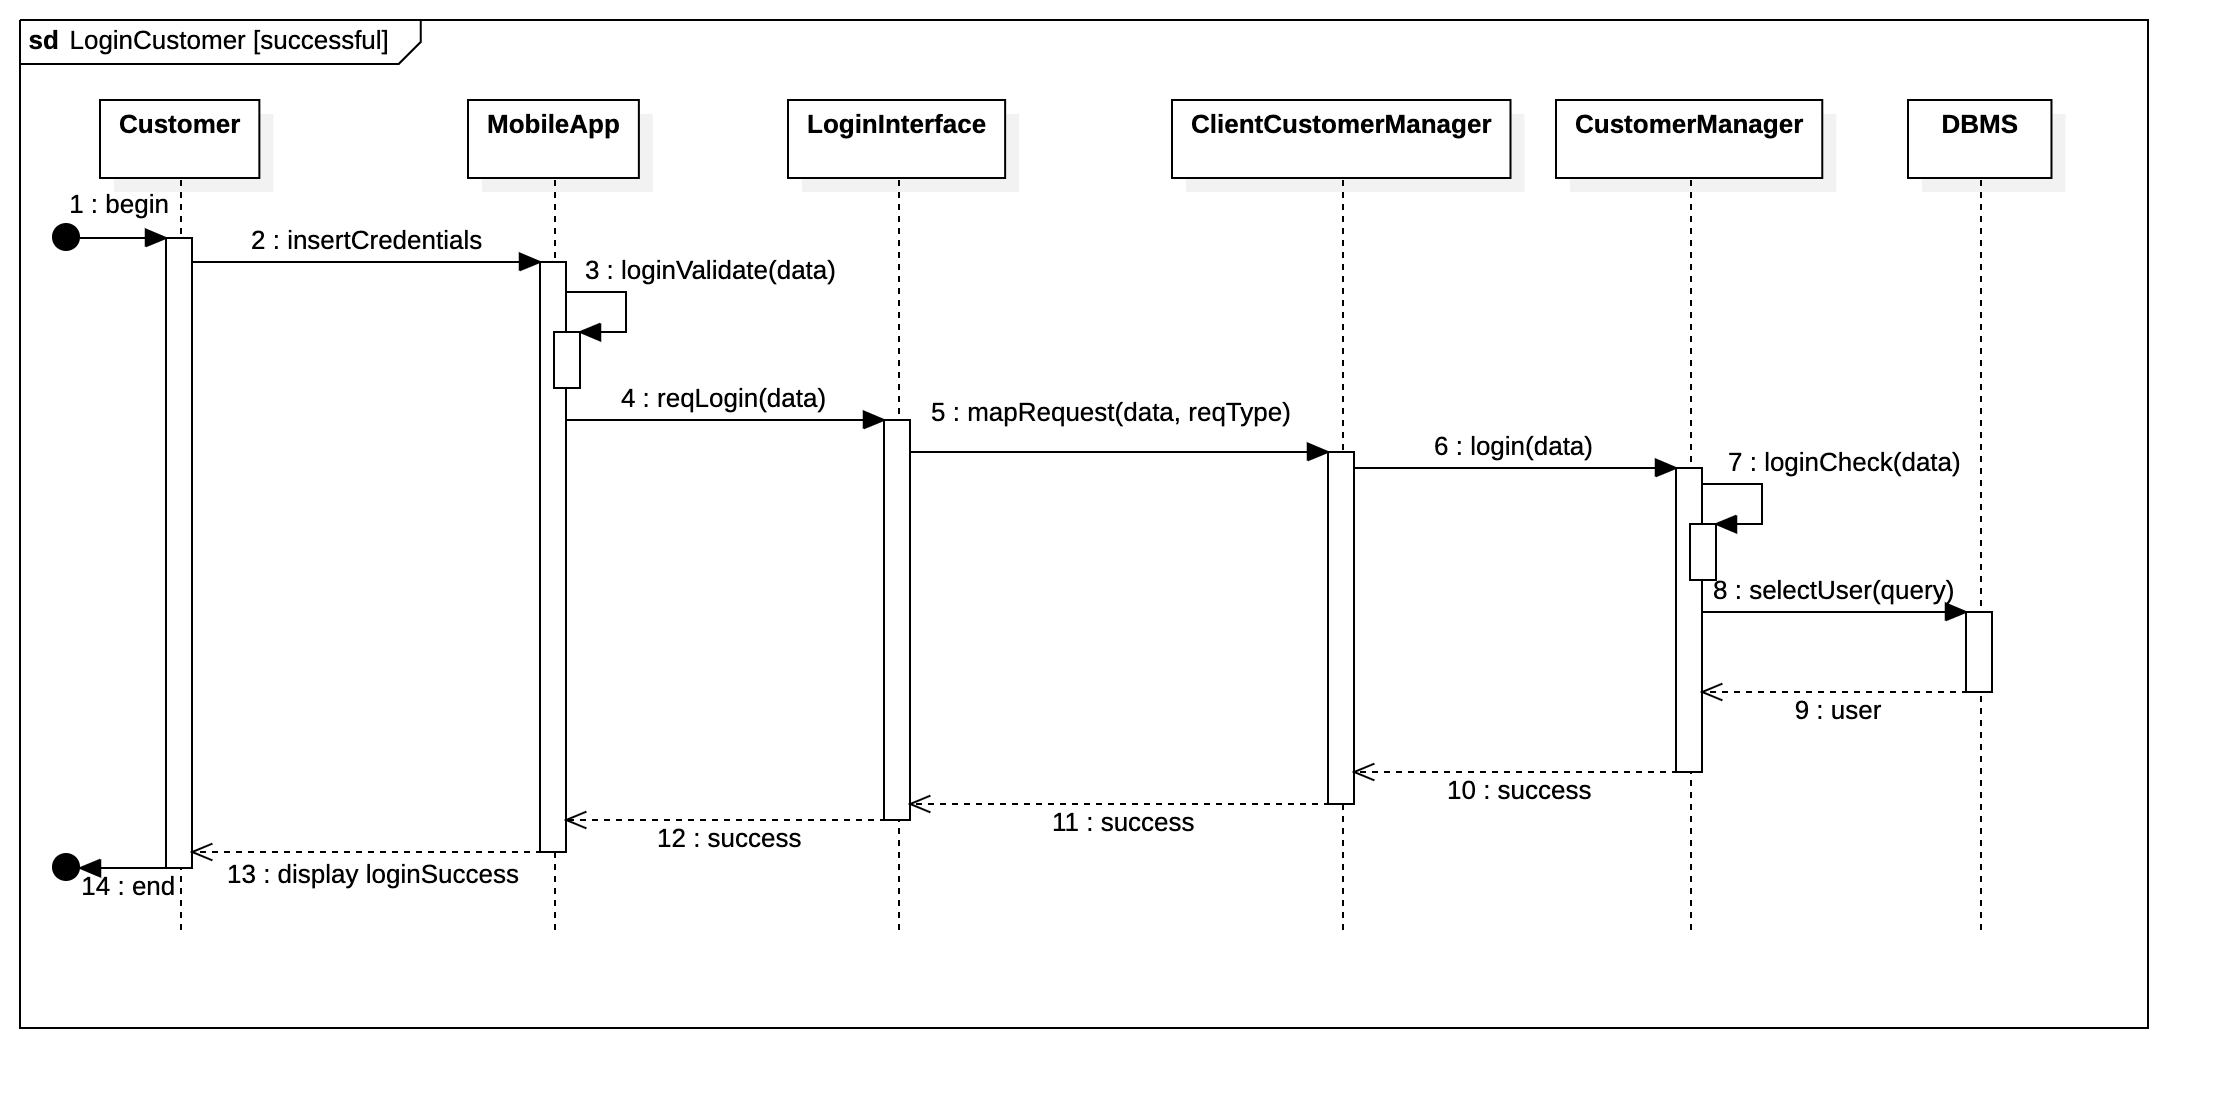
\includegraphics[width=\textwidth]{img/runtime/cust_login_success}
        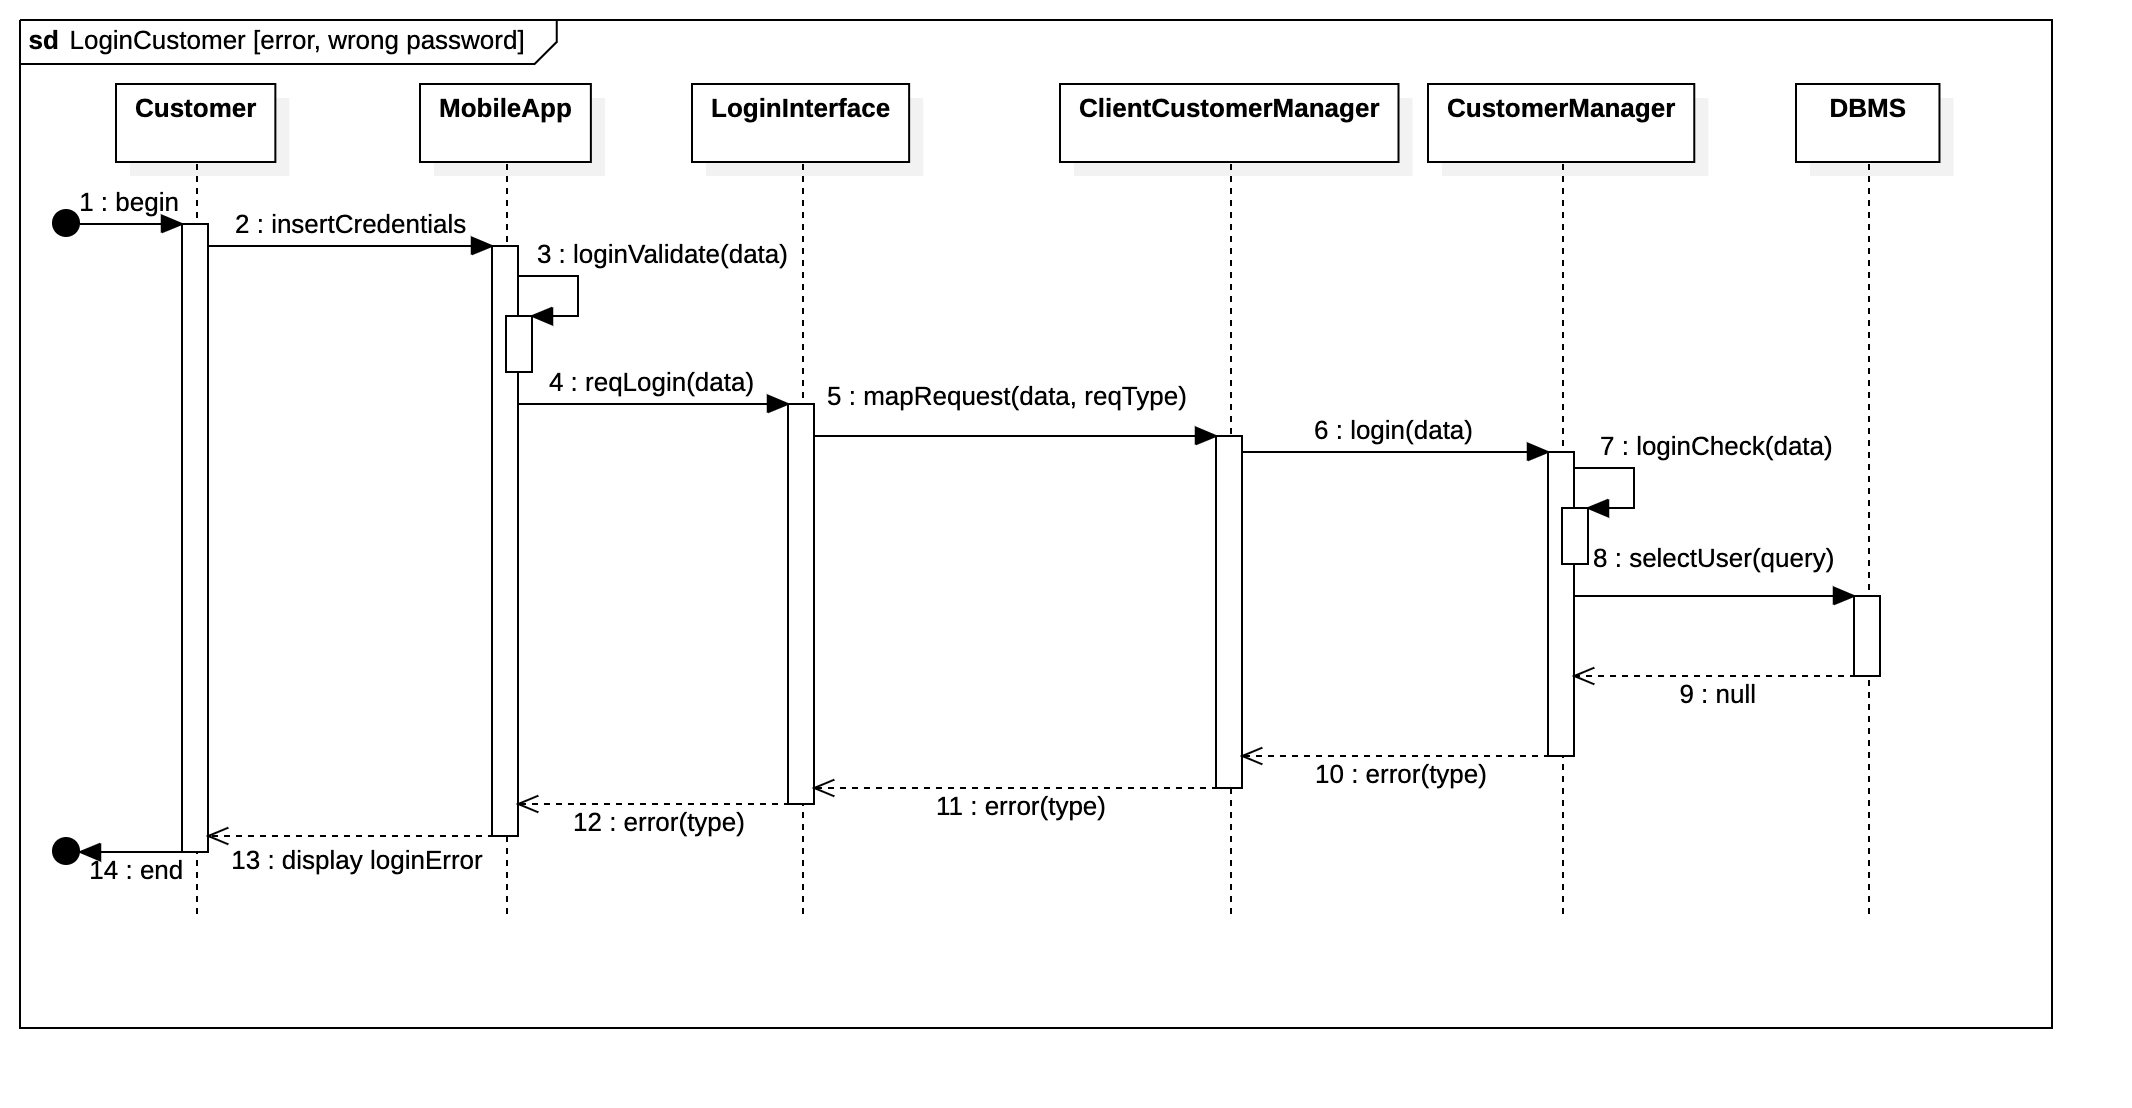
\includegraphics[width=\textwidth]{img/runtime/cust_login_error}
    \end{center}
\end{figure}
The Customer inputs his login credentials and then the MobileApp sends the request, through the LoginInterface to the ClientCustomerManager, which forwards them to the CustomerManager that checks for their correctness and then interrogates the DBMS and searches for the credentials. If the returned value is null the ClientManager sends a specific error message and the login fails, otherwise a 200 response status code is sent to the MobileApp.
\subsubsection{View Nearby Stations}\label{nearby_stations}
\begin{figure}[H]
    \begin{center}
        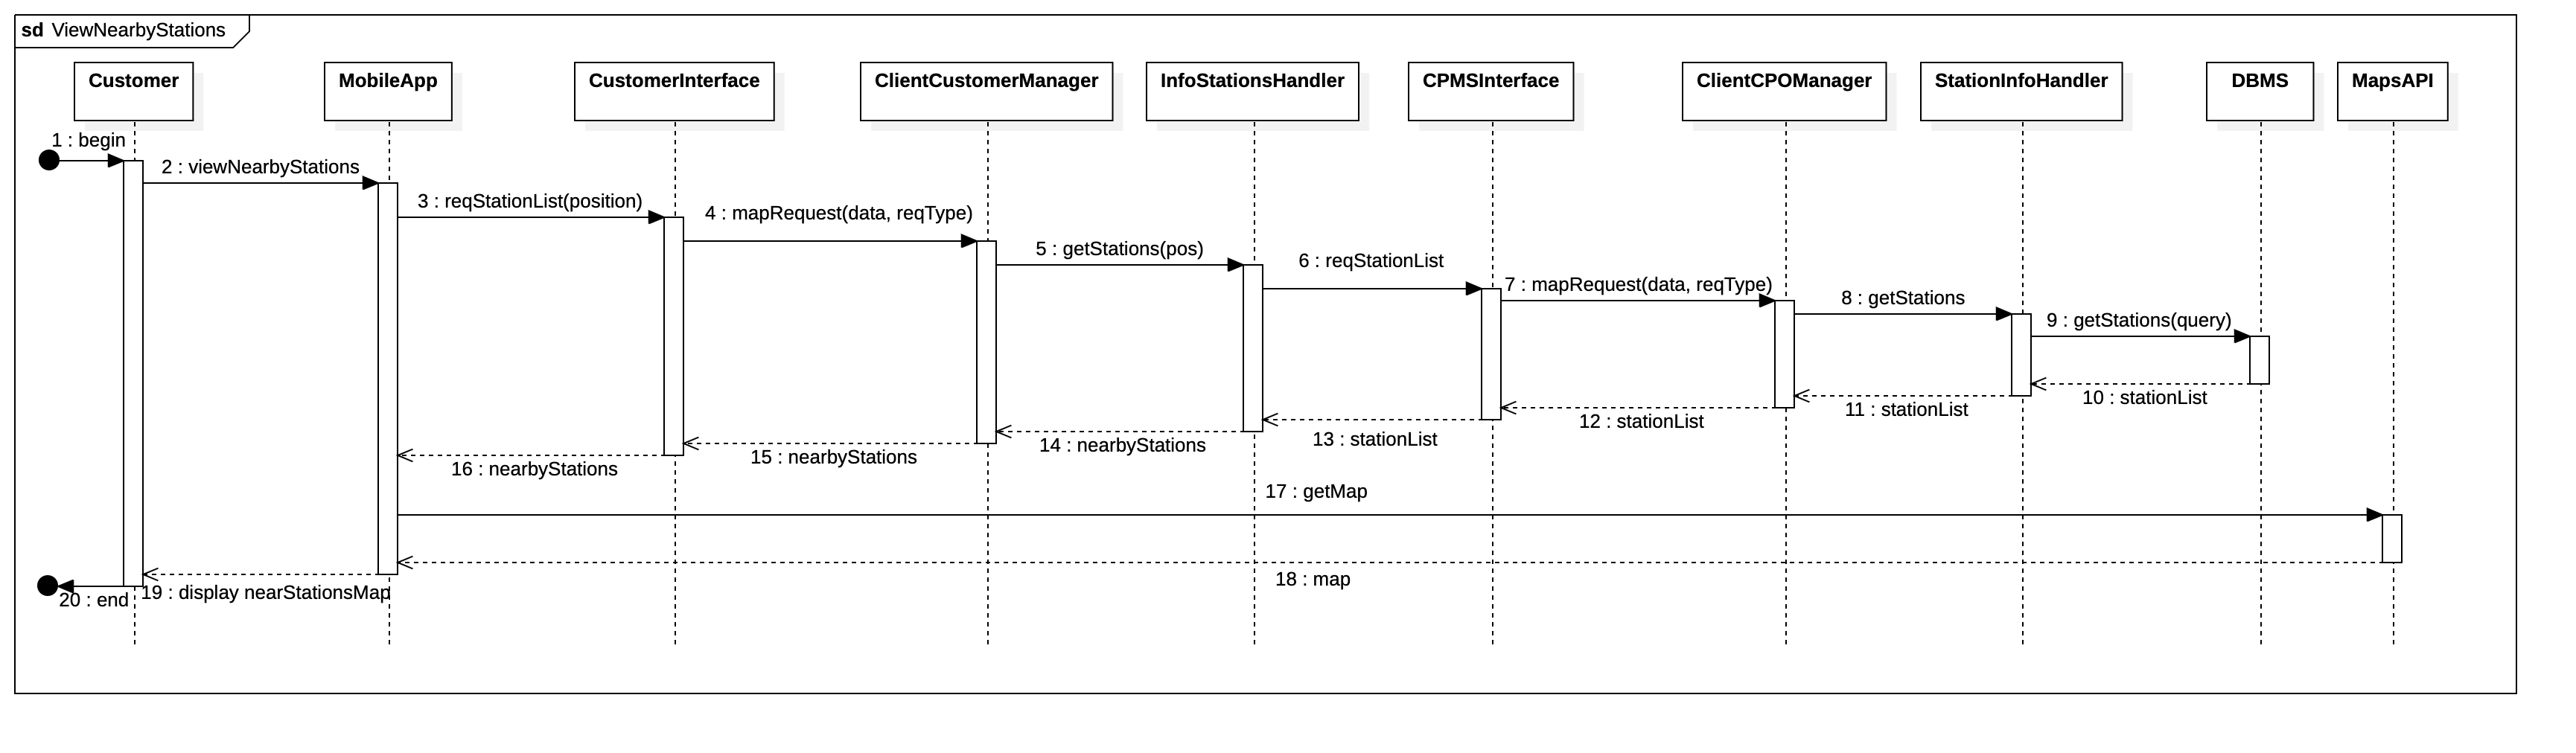
\includegraphics[width=\textwidth]{img/runtime/nearby_stations}
    \end{center}
\end{figure}
To access this view it is necessary to have performed the login before (\ref{cust_login}). The MobileApp will automatically request the list of stations that are nearby the Customer, through the CustomerInterface to the ClientCustomerManager, which forwards them to the InfoStationsHandler. The InfoStationsHandler will then request the list of stations by contacting the CPMS subsystem (Module 2). The CPMS subsystem functions can be accessed by contacting the CPMSInterface. In this case, the ClientCPOManager will forward the request to the StationInfoHandler, which will ultimately access the CPMS' DBMS. The InfoStationsHandler will then filter the far stations and will return to the MobileApp the list of close stations, that will be used in conjunction with the MapsAPI by the app, in order display an interactive map to the customer to the Customer.
\subsubsection{View Information about a Station}
\begin{figure}[H]
    \begin{center}
        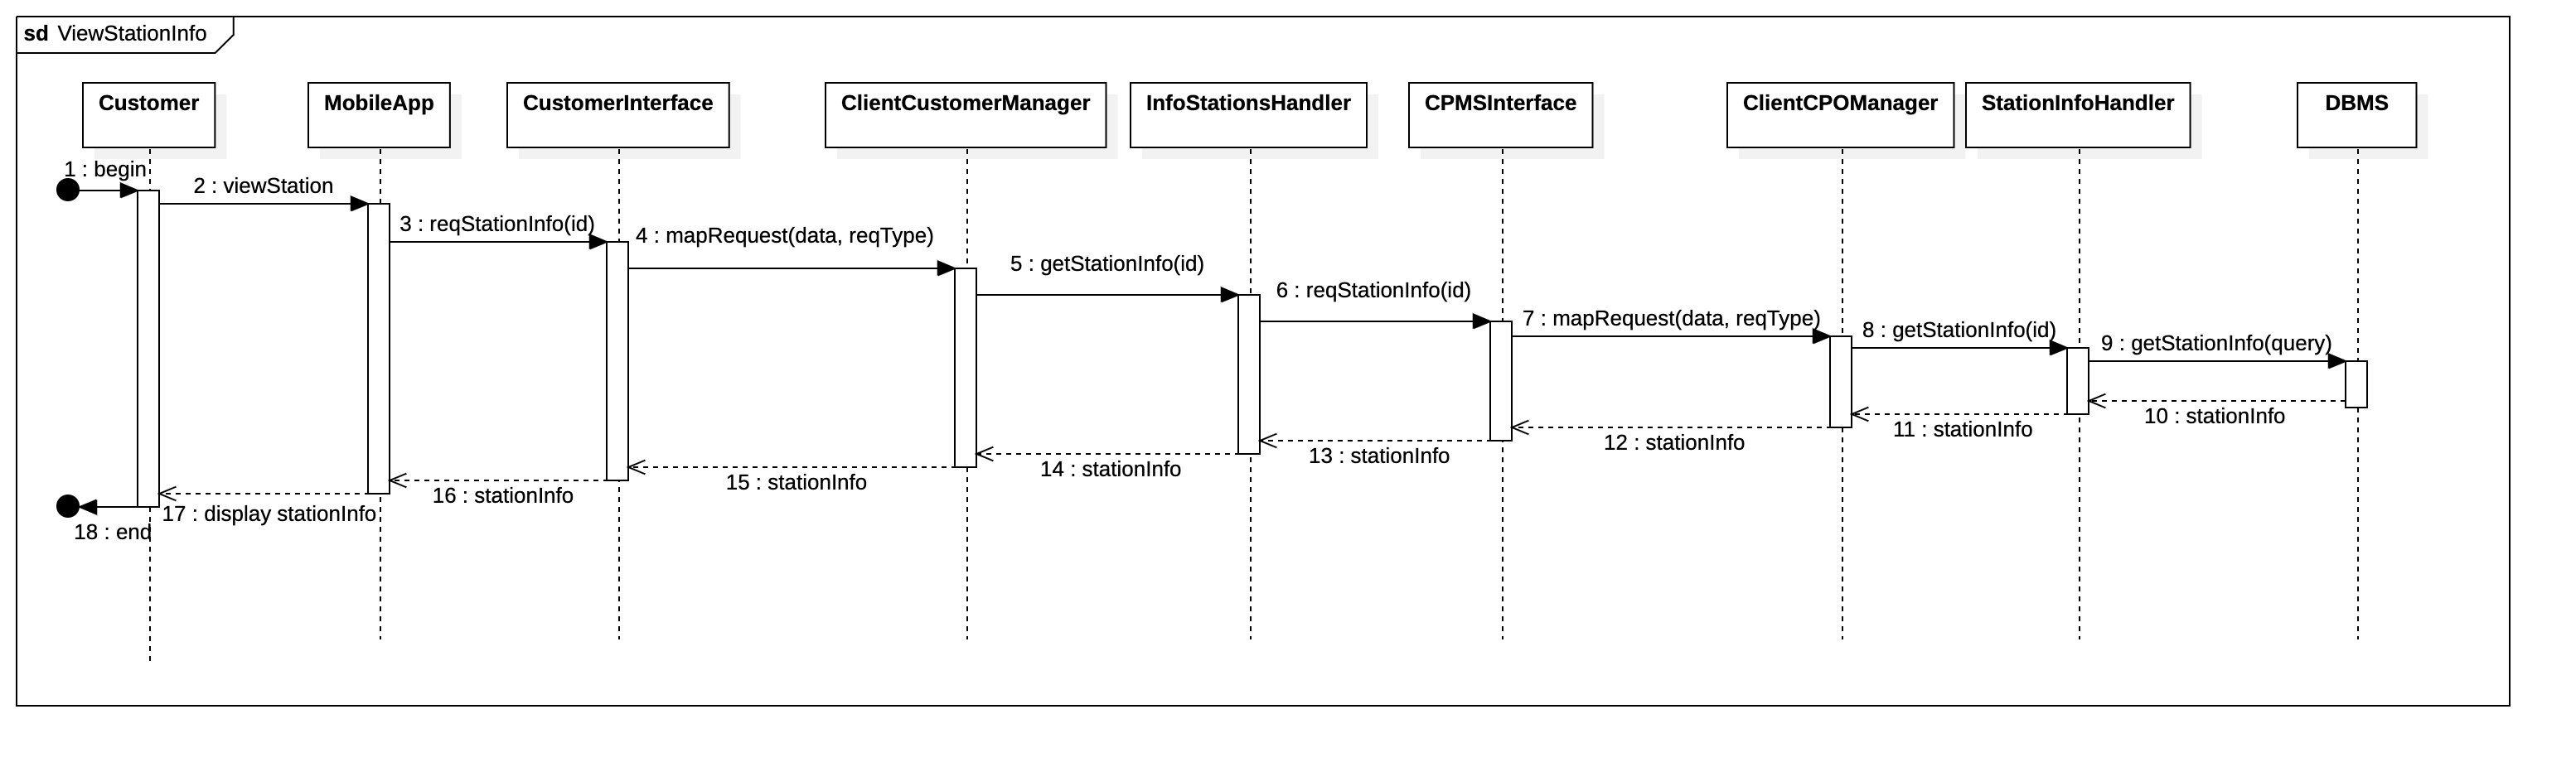
\includegraphics[width=\textwidth]{img/runtime/station_info}
    \end{center}
\end{figure}
To access this view it is necessary to have performed the login before (\ref{cust_login}). This view is accessed when the "Book" button from the View Nearby Stations View (\ref{nearby_stations}) is selected. The MobileApp will send the booking request of the selected charging station through the CustomerInterface to the ClientCustomerManager, which forwards them to the InfoStationsHandler. The InfoStationsHandler will then request the list of stations by contacting the CPMS subsystem (Module 2). The CPMS subsystem functions can be accessed by contacting the CPMSInterface. In this case, the ClientCPOManager will forward the request to the StationInfoHandler, which will ultimately access the CPMS' DBMS. The MobileApp will then receive the information of the selected station, that will be displayed to the Customer.
\subsubsection{Book a Charge}\label{book_charge}
\begin{figure}[H]
    \begin{center}
        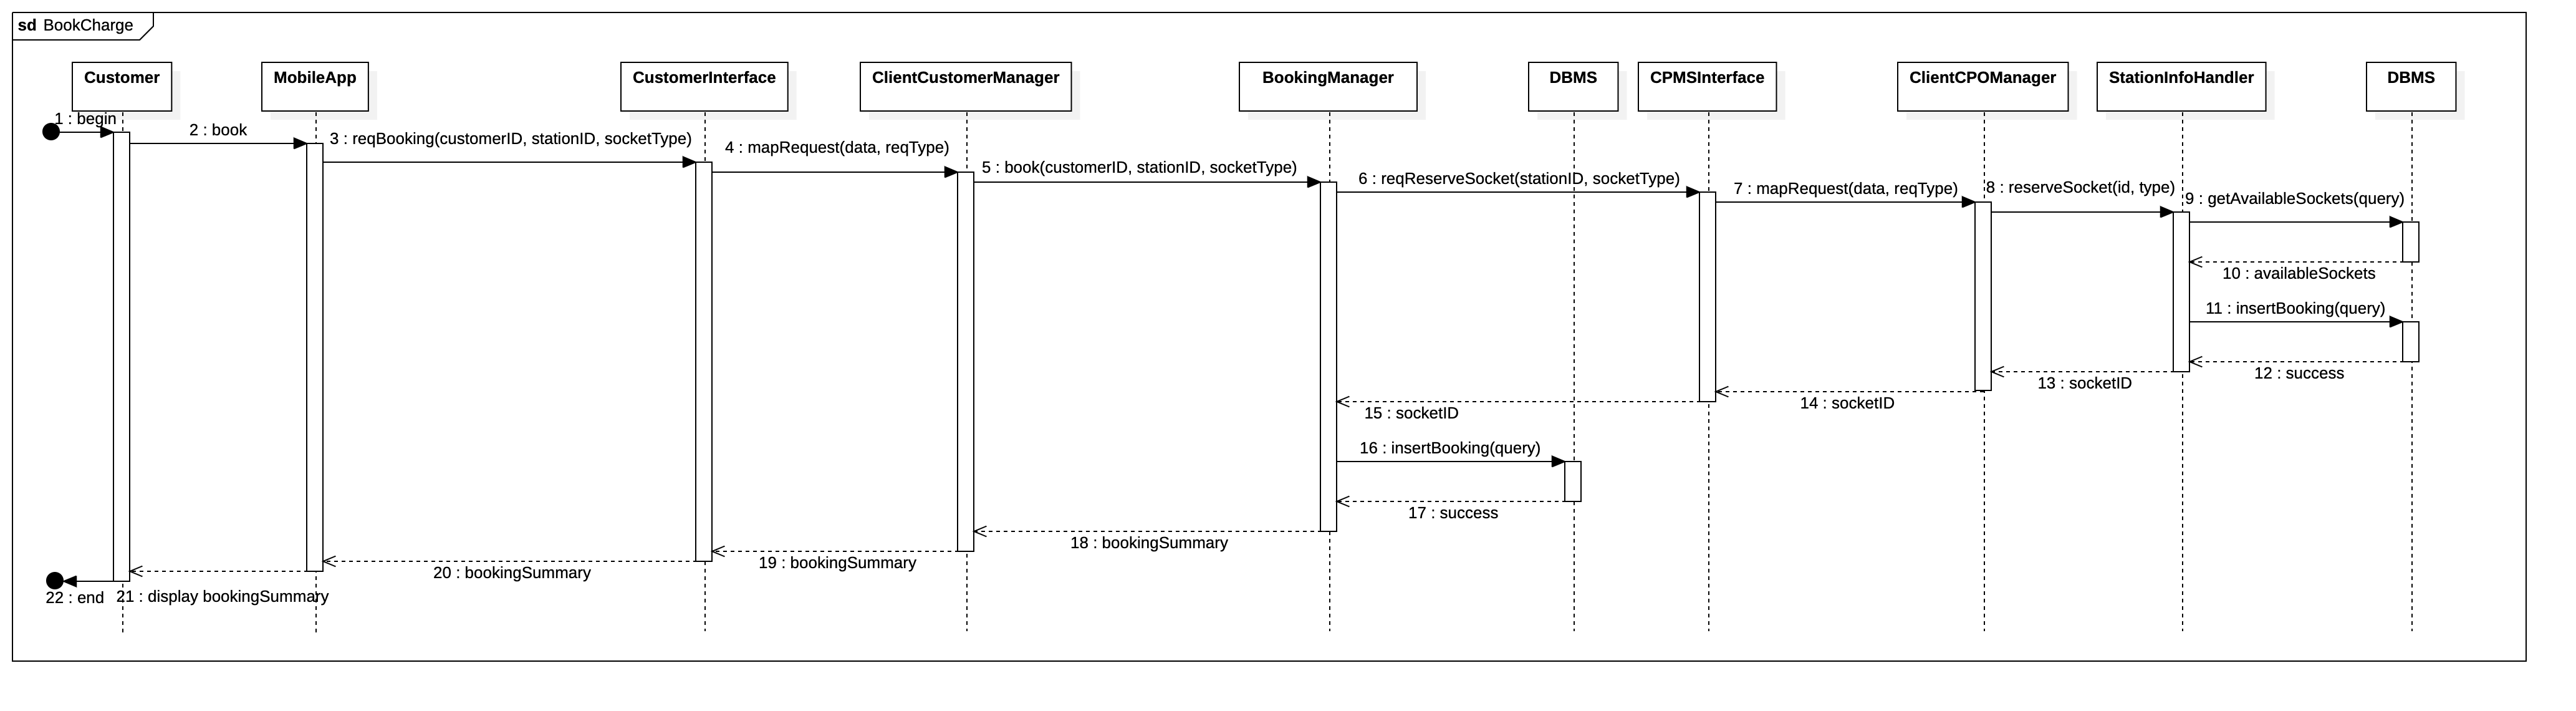
\includegraphics[width=\textwidth]{img/runtime/book_charge}
    \end{center}
\end{figure}
To access this view it is necessary to have performed the login before (\ref{cust_login}). This view is accessed when the "Book" button from the View Information about a Station (\ref{nearby_stations}) is selected. The MobileApp will request the booking of the selected type of socket from the current charging station through the CustomerInterface to the ClientCustomerManager, which forwards the request to the BookingManager. The BookingManager will then request the socket by contacting the CPMS subsystem (Module 2). The CPMS subsystem functions can be accessed by contacting the CPMSInterface. In this case, the ClientCPOManager will forward the request to the StationInfoHandler, which will ultimately access the CPMS' DBMS, where a list of the available sockets will be retrieved, and then the socket will be picked and inserted. If successful, the CPMS subsytem will return the 200 status to the BookingManager, that will store all the booking's information on the eMSP's DBMS. The MobileApp will then display a message stating that the charge has started.
\subsubsection{Start Charging}\label{start_charge}
\begin{figure}[H]
    \begin{center}
        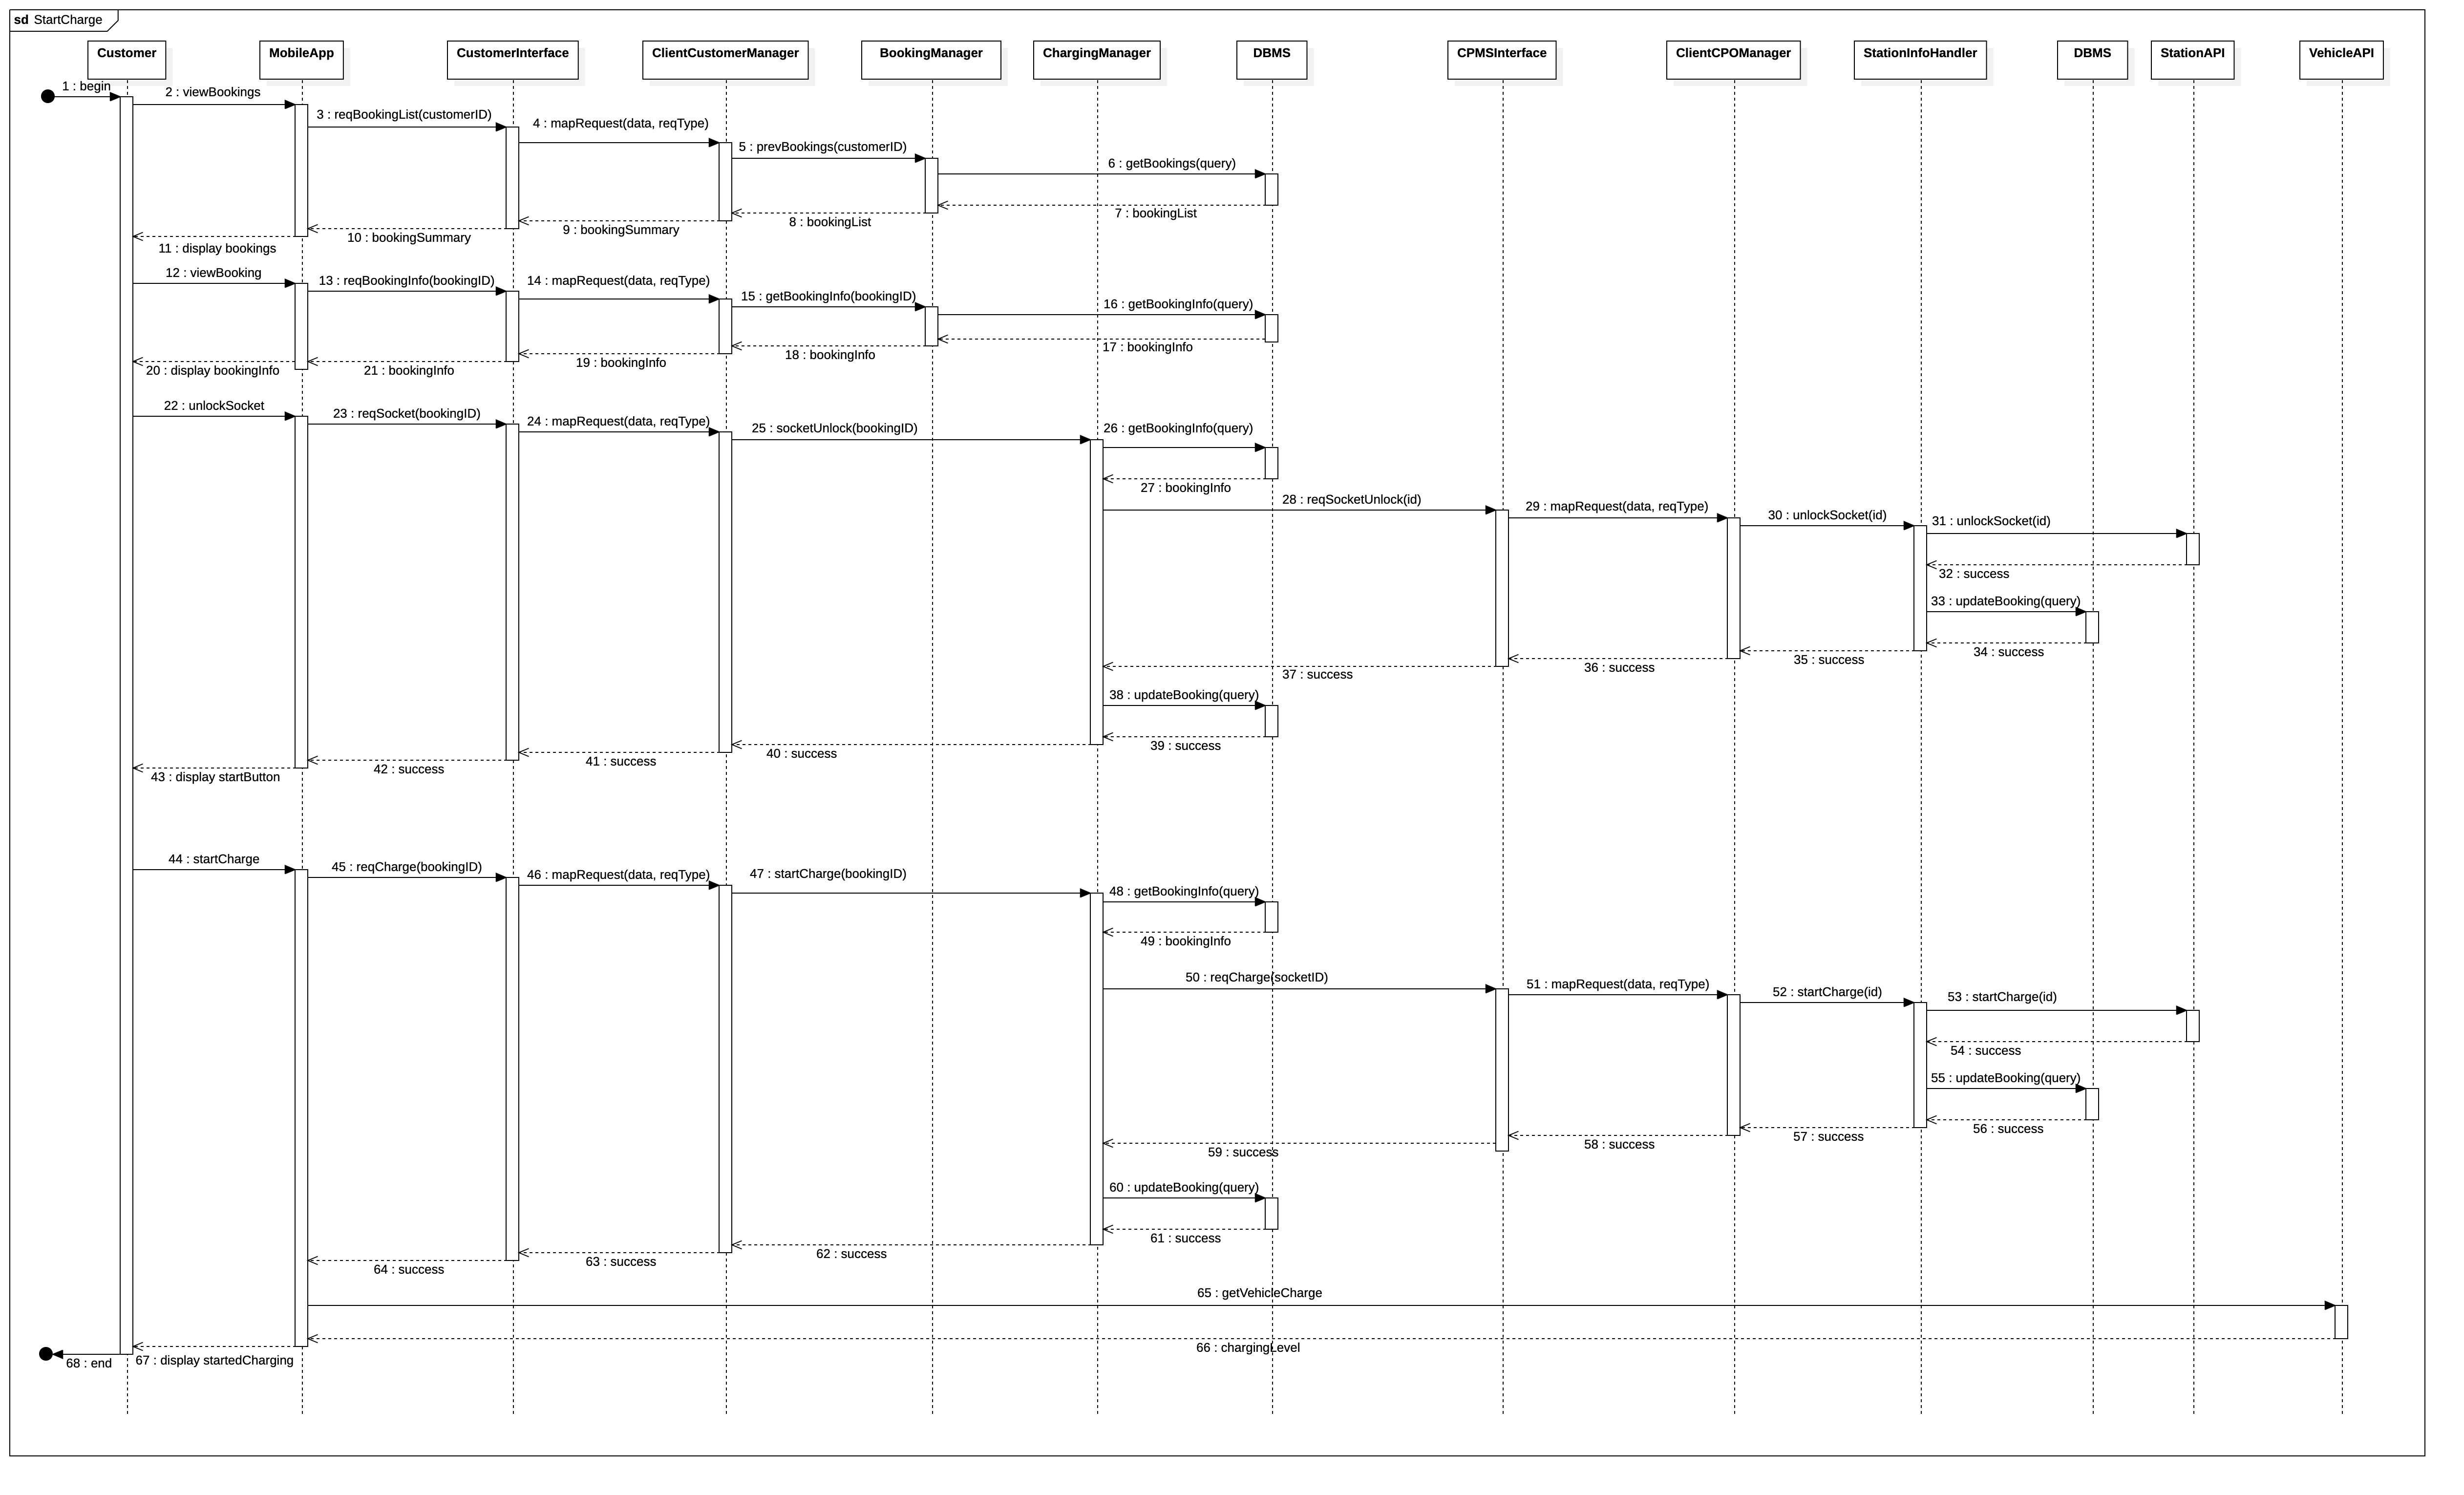
\includegraphics[width=\textwidth]{img/runtime/start_charge}
    \end{center}
\end{figure}
To access this view it is necessary to have performed the login before (\ref{cust_login}). The Customer must access the Bookings View. The MobileApp will then request the list of performed booking of the Customer through the CustomerInterface to the ClientCustomerManager, which forwards the request to the BookingManager. Finally, the BookingManager will access the DBMS in order to retrieve the list of previous bookings, that will then be displayed to the Customer. When a specific booking is selected, the App will contact the BookingManger again similarly as before, only this time to request the specific information of a booking, that will then be displayed to the user. Now, the Customer can select the "Unlock socket" button, that will trigger the ChargingManager similarly to the BookingManager previously explained, but then will contact the CPMS subsystem (Module 2) in order to unlock the socket through the StationInfoHandler and the external StationAPI, that will perform the physical socket unlock, and the status will be recorded on both the eMSP and the CPMS DBMS. In the end, the Customer view will be updated, and now the "Start Charging" button will appear only when the physical connection between the vehicle and the socket has been established. When the button is pressed and the requirements are met, the ChargingManager will then request the start of the charging by contacting the CPMS subsystem. The StationInfoHandler, will request the start of the charge to the Station API, and then will ultimately access the CPMS' DBMS to store the state update. The CPMS subsytem will return the specific socketID to the BookingManager, that will store all the booking's information on the eMSP's DBMS. The MobileApp will then receive the summary of the booking, that will be displayed to the Customer.
\subsubsection{Pay for the Charging Service}
\begin{figure}[H]
    \begin{center}
        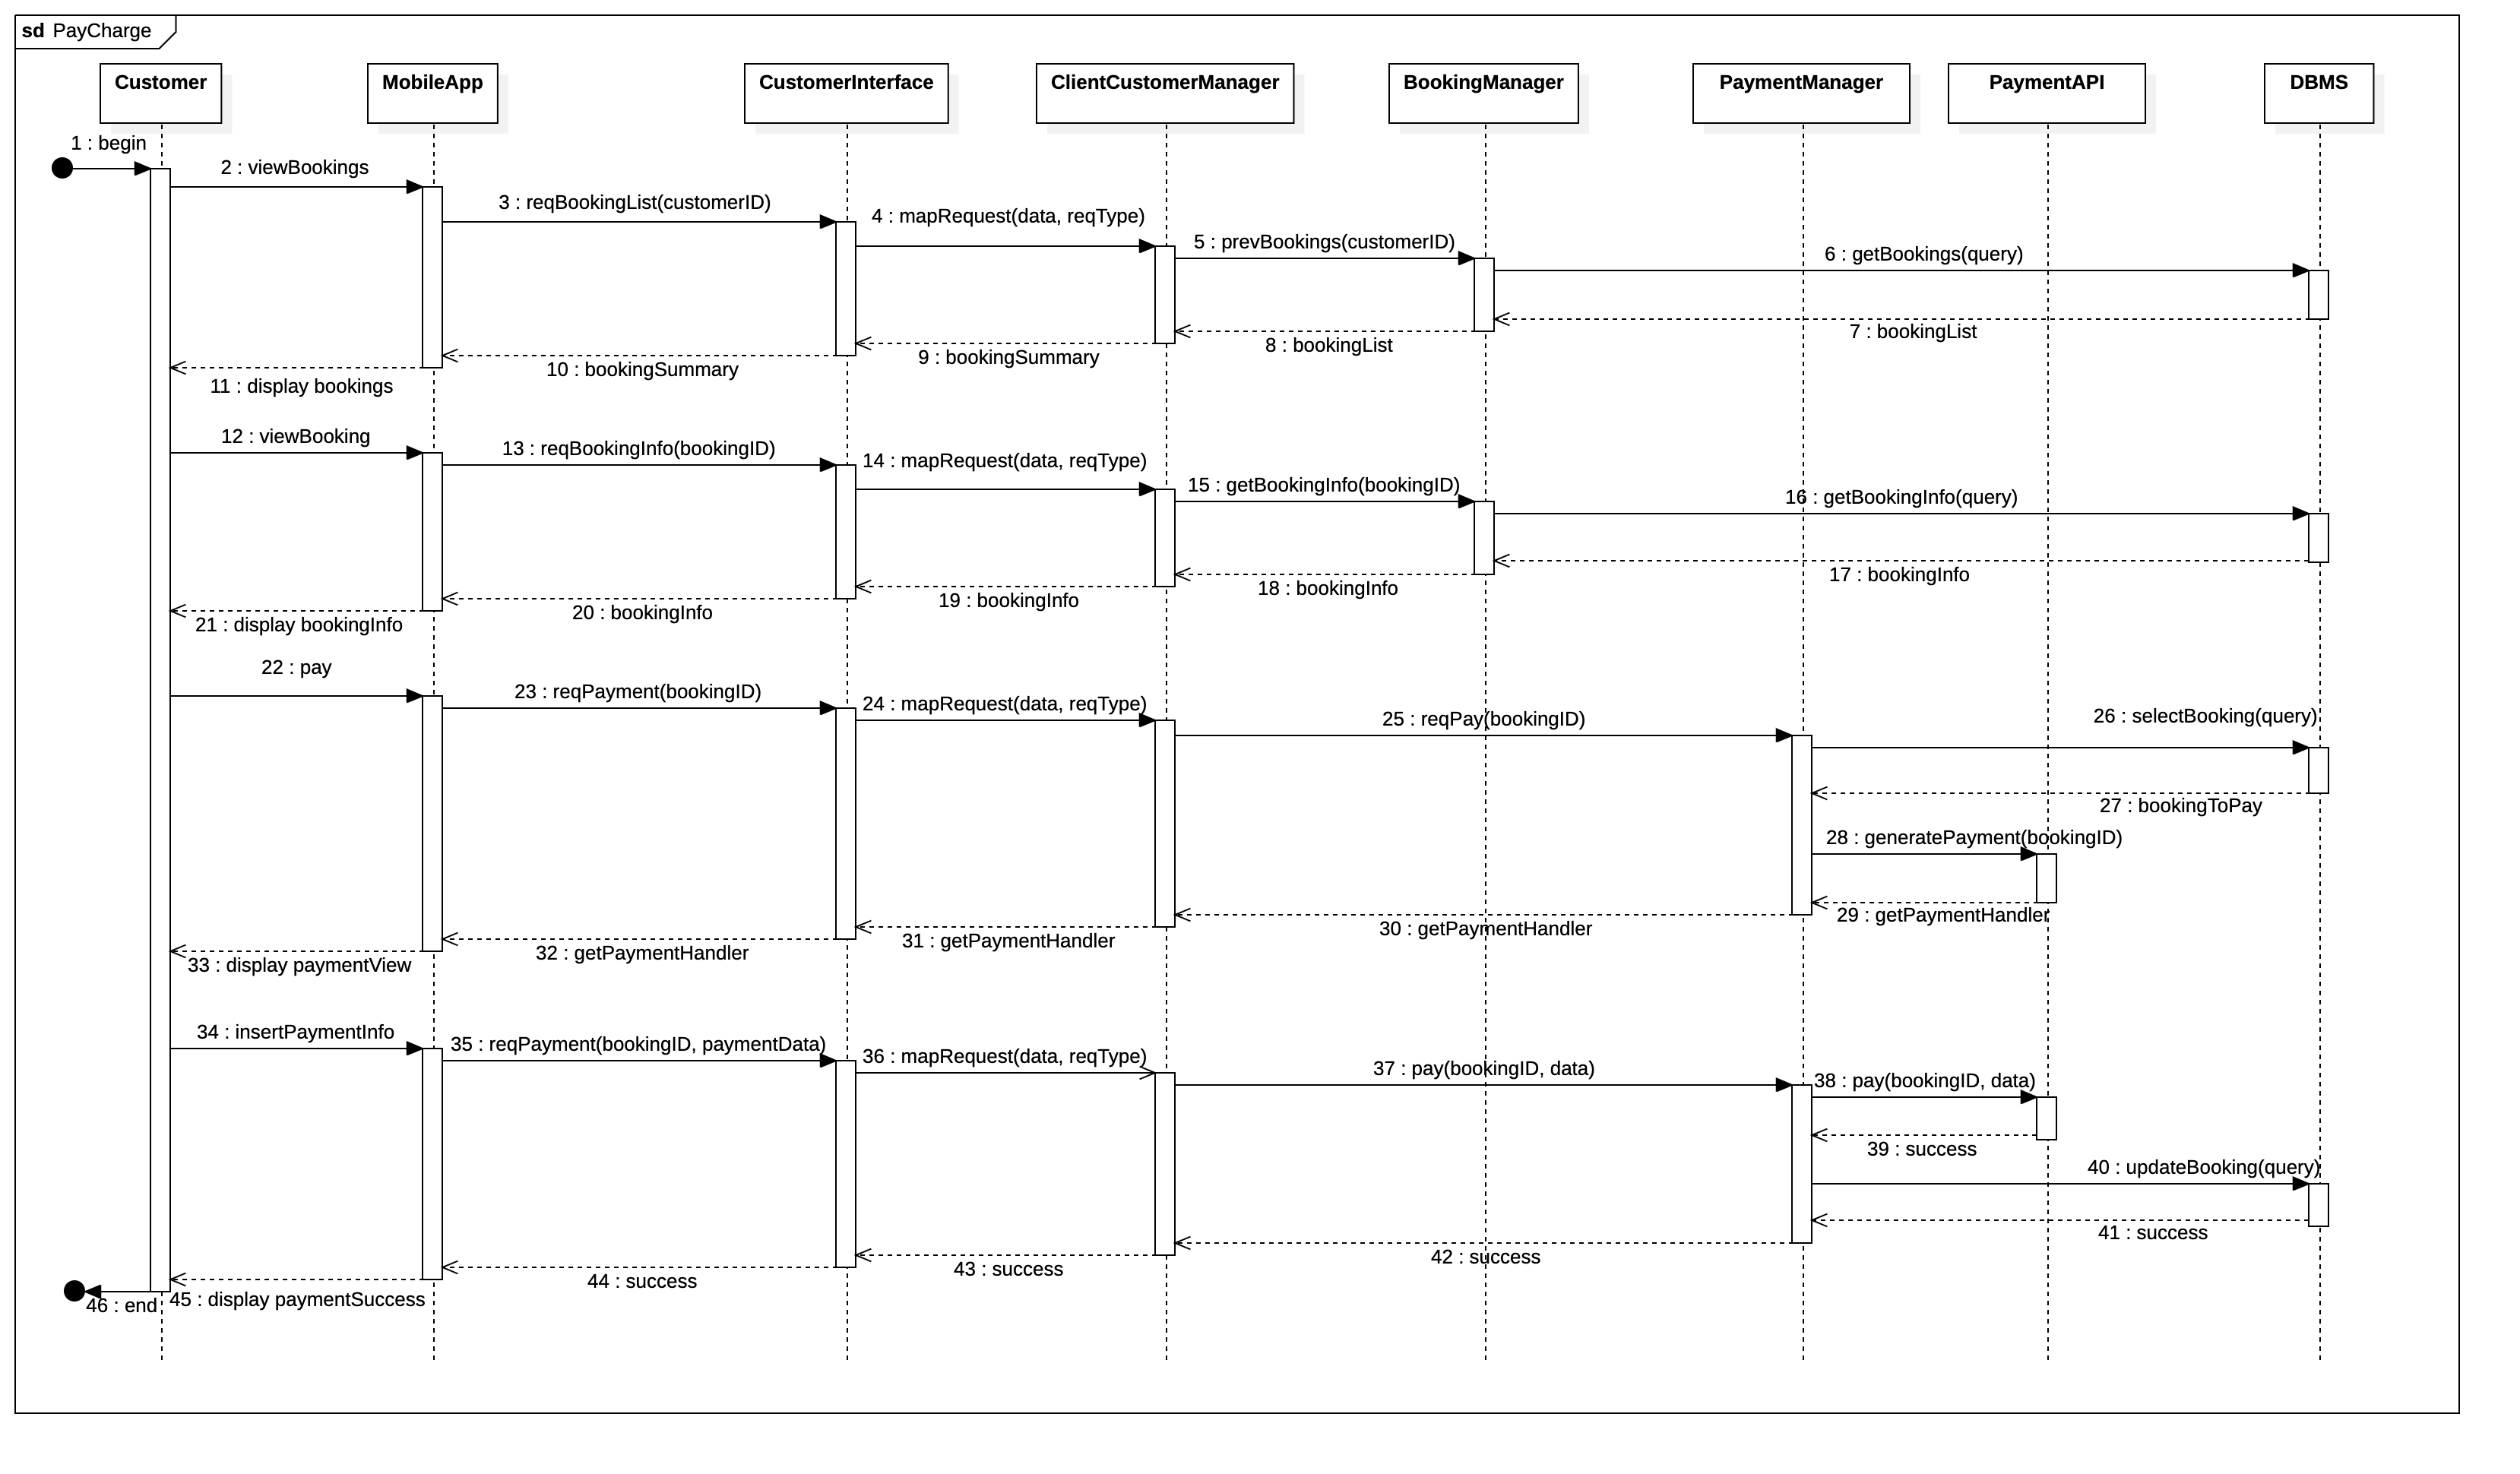
\includegraphics[width=\textwidth]{img/runtime/pay_charging}
    \end{center}
\end{figure}
To access this view it is necessary to have performed the login before (\ref{cust_login}). The Customer must access the Bookings View and a specific booking in a similarly to Start Charging(\ref{start_charge}). The MobileApp will then request the generation of a payment ticked through the CustomerInterface to the ClientCustomerManager, which forwards the request to the PaymentManager that will access the PaymentAPI. The Customer will be presented with a web page inside the app where he can pay with whatever method the payment processor offer. It is important to say that this web template will be provided and mantained by the external payment service. After the Customer has input his information, the MobileApp will contact the PaymentManager again, that will forward the information to the PaymentAPI for processing. If correct, the 200 OK status code is returned.
\subsection{Change active vehicle for suggestions}
\begin{figure}[H]
    \begin{center}
        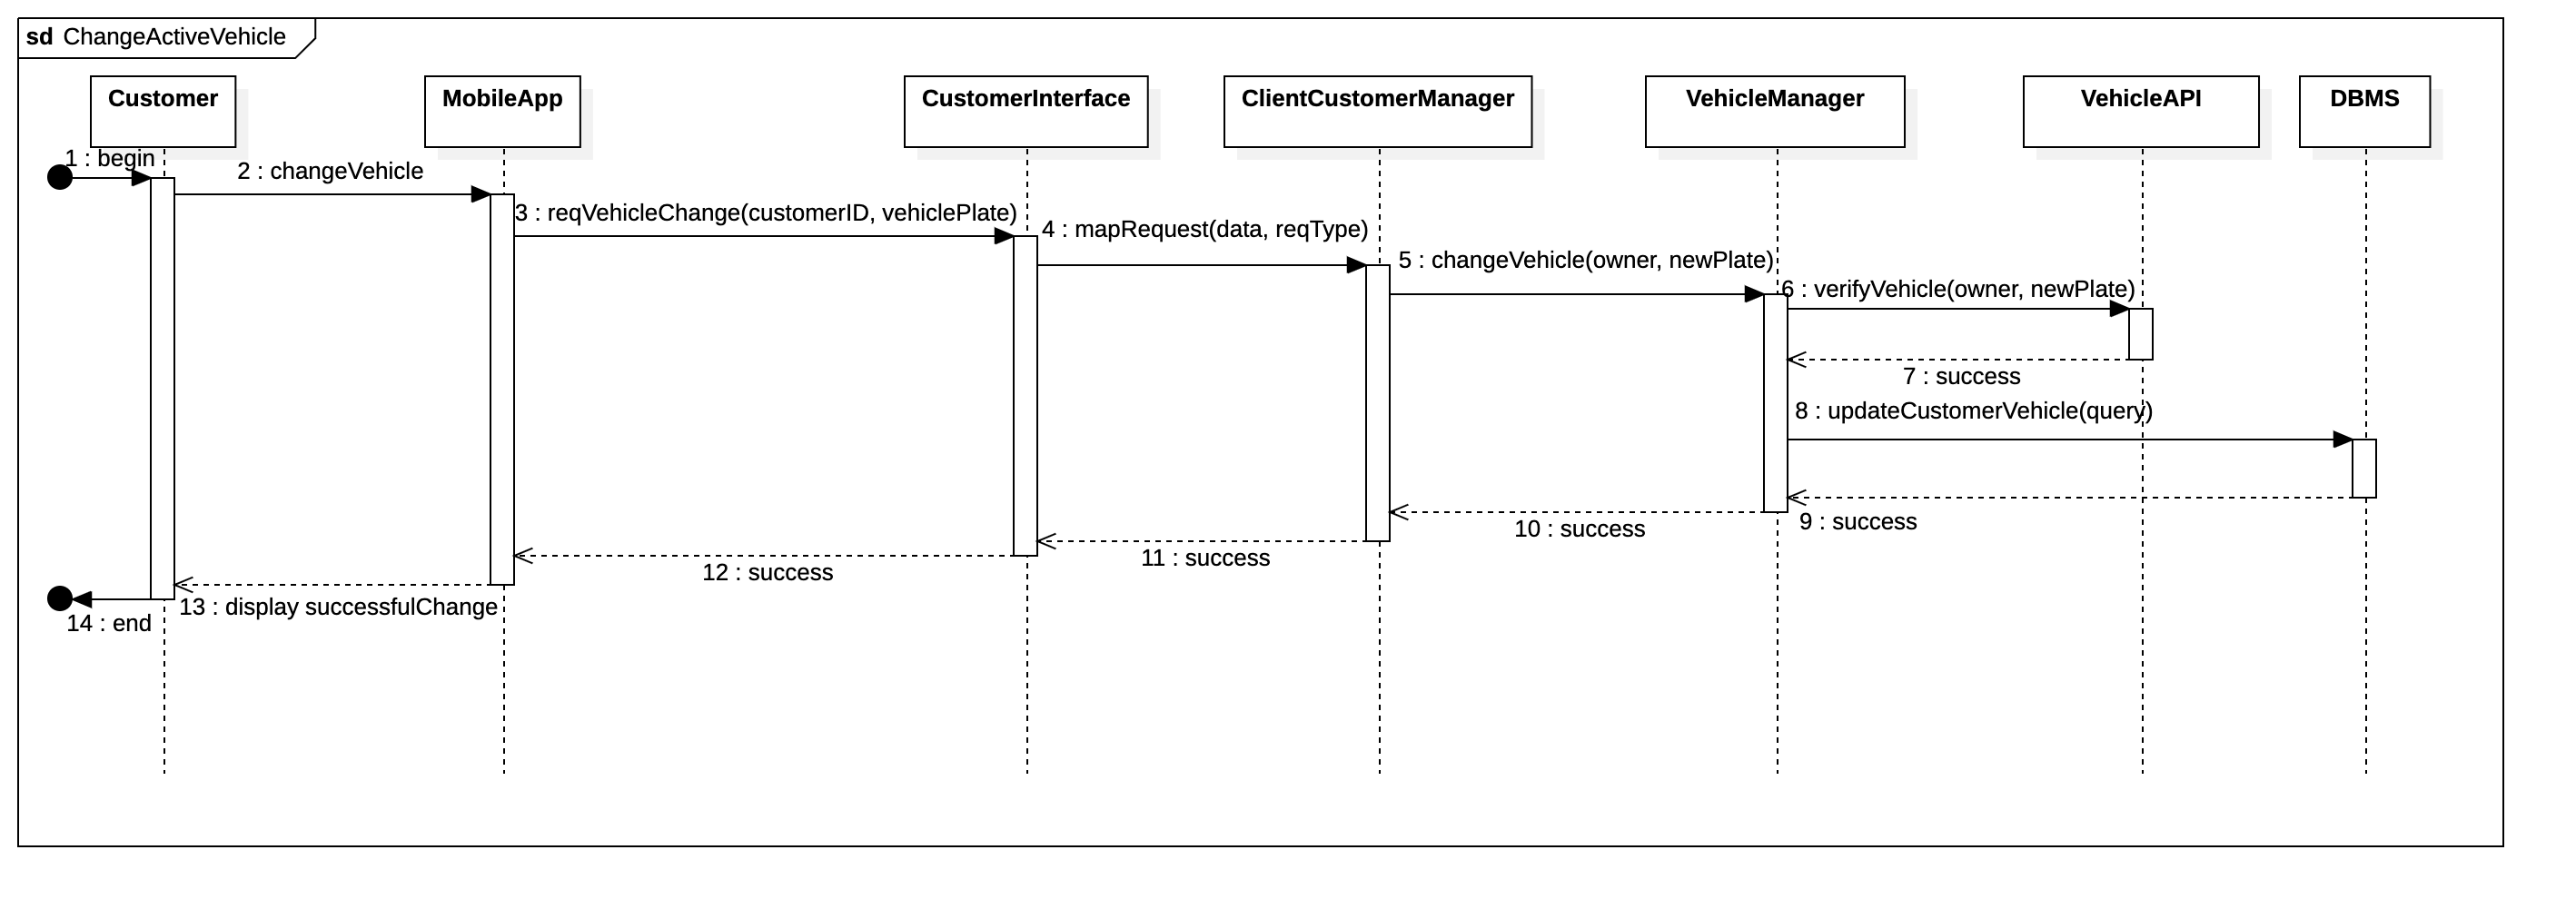
\includegraphics[width=\textwidth]{img/runtime/change_vehicle.png}
    \end{center}
\end{figure}
To access this view it is necessary to have performed the login before (\ref{cust_login}). The MobileApp, after the Customer has input his new license plate, will contact the VehicleManager through the CustomerInterface and the ClientCustomerManager. The VehicleManager will then verify the ownership and the plate itself through the external VehicleAPI. If successful, the updated is stored on the DBMS and the 200 OK status code is returned to the MobileApp.
\subsubsection{Book a charge from a suggestion}
\begin{figure}[H]
    \begin{center}
        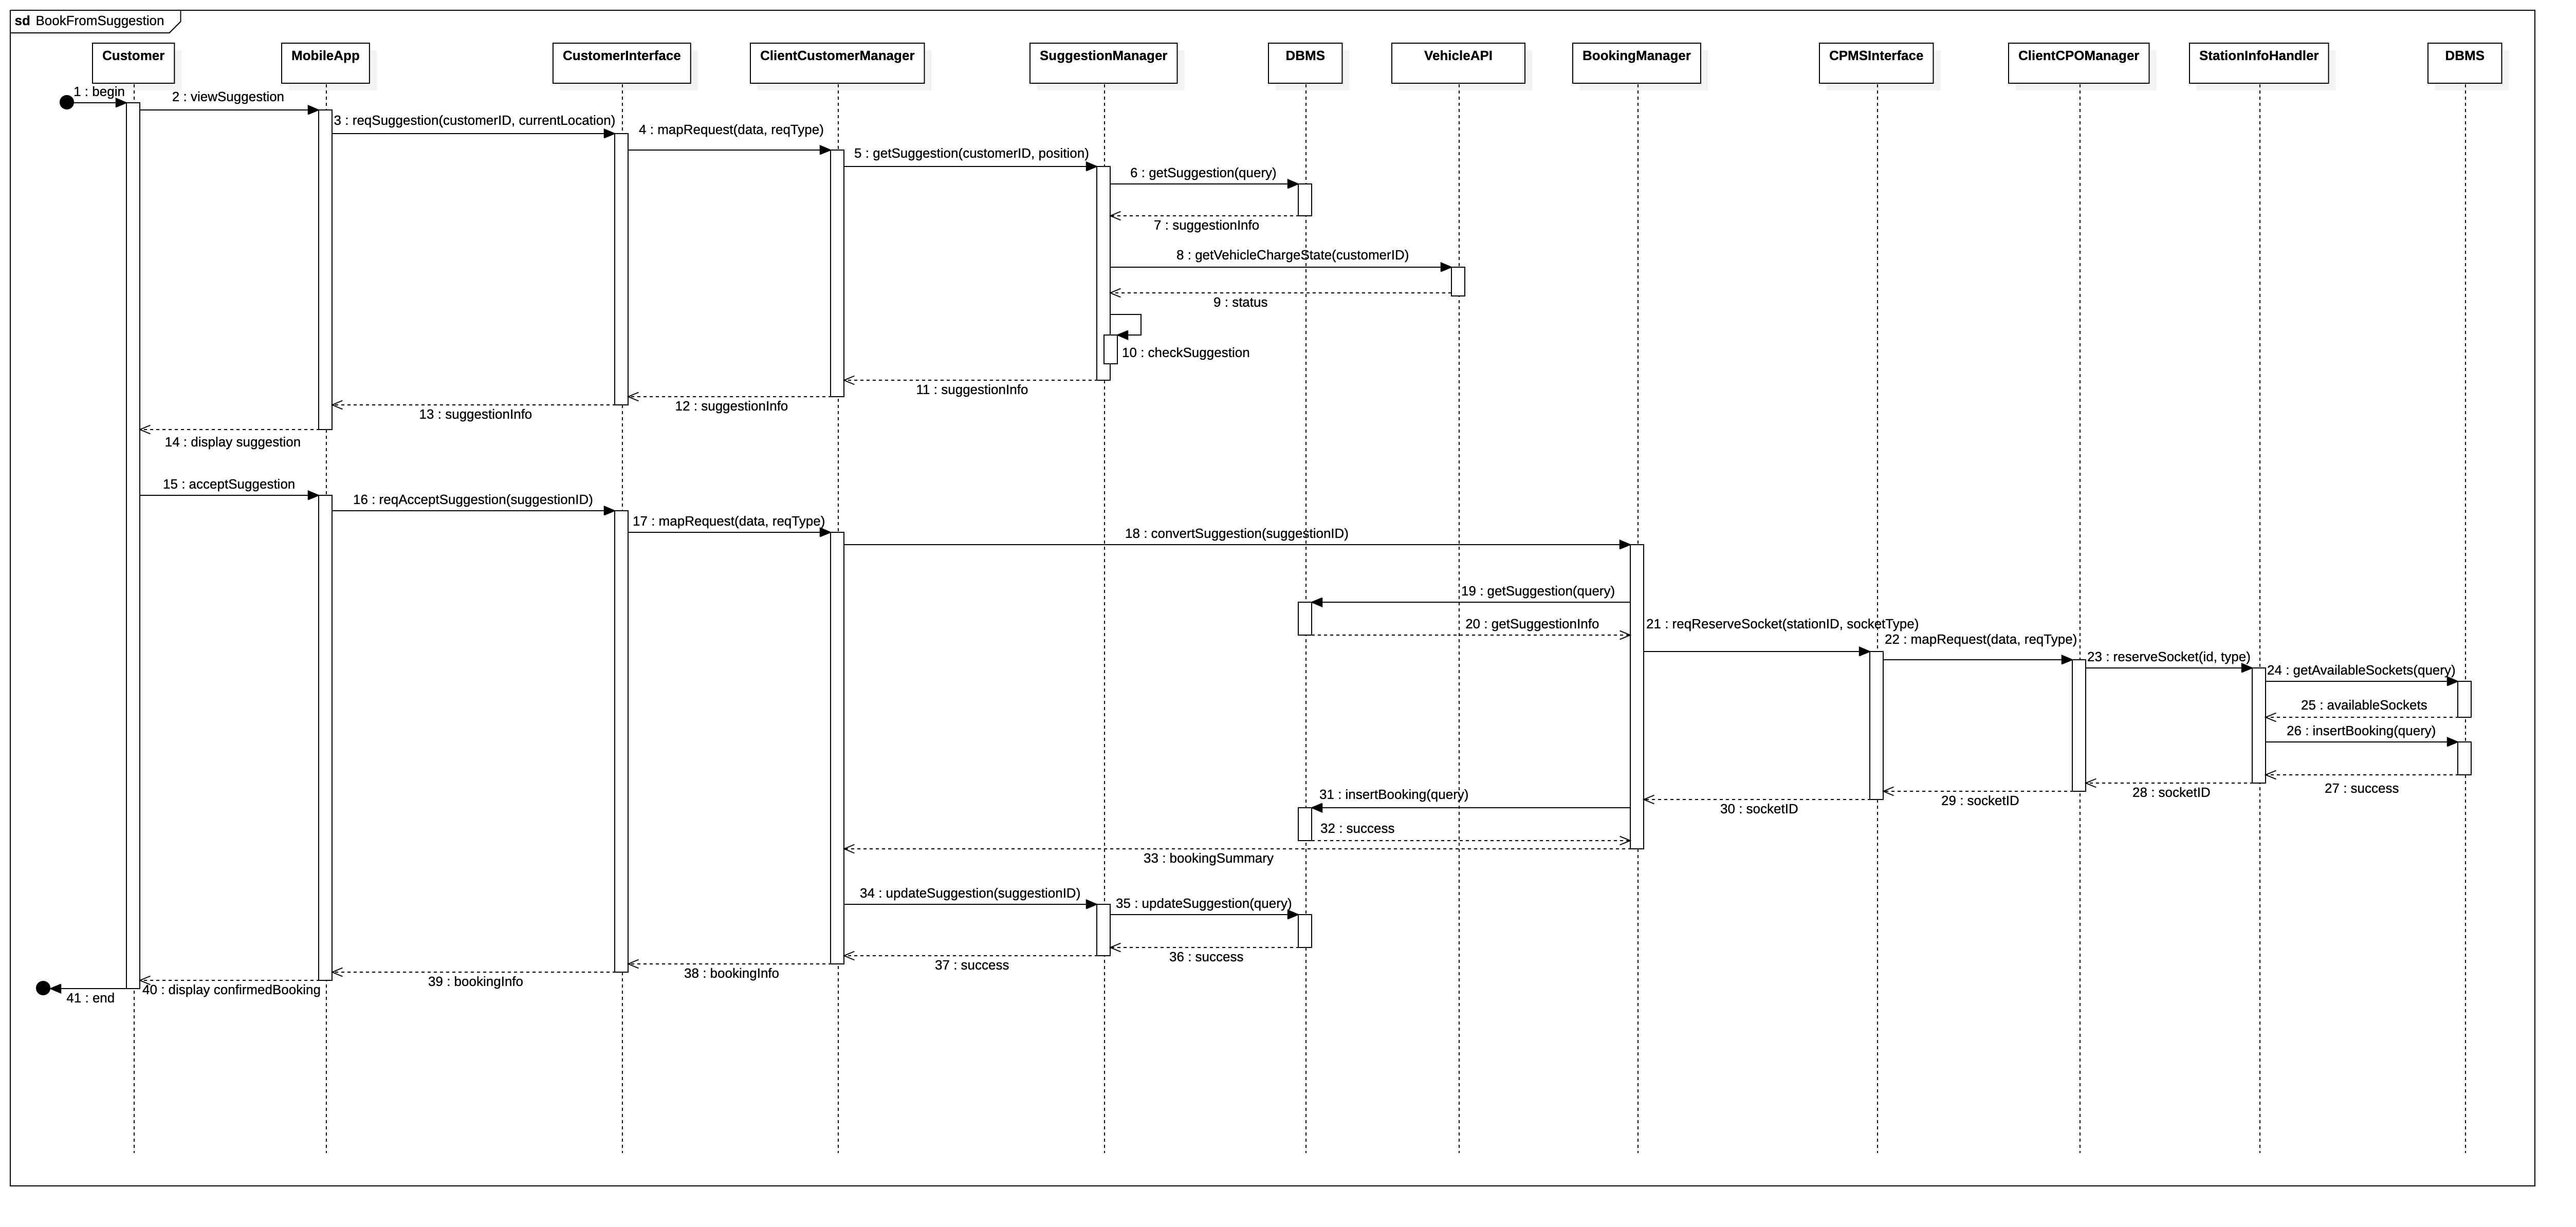
\includegraphics[width=\textwidth]{img/runtime/suggestion.png}
    \end{center}
\end{figure}
To access this view it is necessary to have performed the login before (\ref{cust_login}). When a Customer clicks on a received push notification, the MobileApp will contact the SuggestionManager that will retrieve the suggestion from the DBMS, and then the vehicle charge state will be retrieved from the CPMS. The SuggestionManager will then check in the suggestion is still valid. If it is still valid, the suggestionInfo will be sent to the MobileApp and displayed to the user. If the Customer accepts the suggestion, the BookingManager will be contacted, and it will retrieve all the suggestion info from the DBMS, and then will perform the booking of a charge in the same way as the Book a Charge view (\ref{book_charge}).
\subsubsection{Login CPO operator}\label{cpo_login}
\begin{figure}[H]
    \begin{center}
        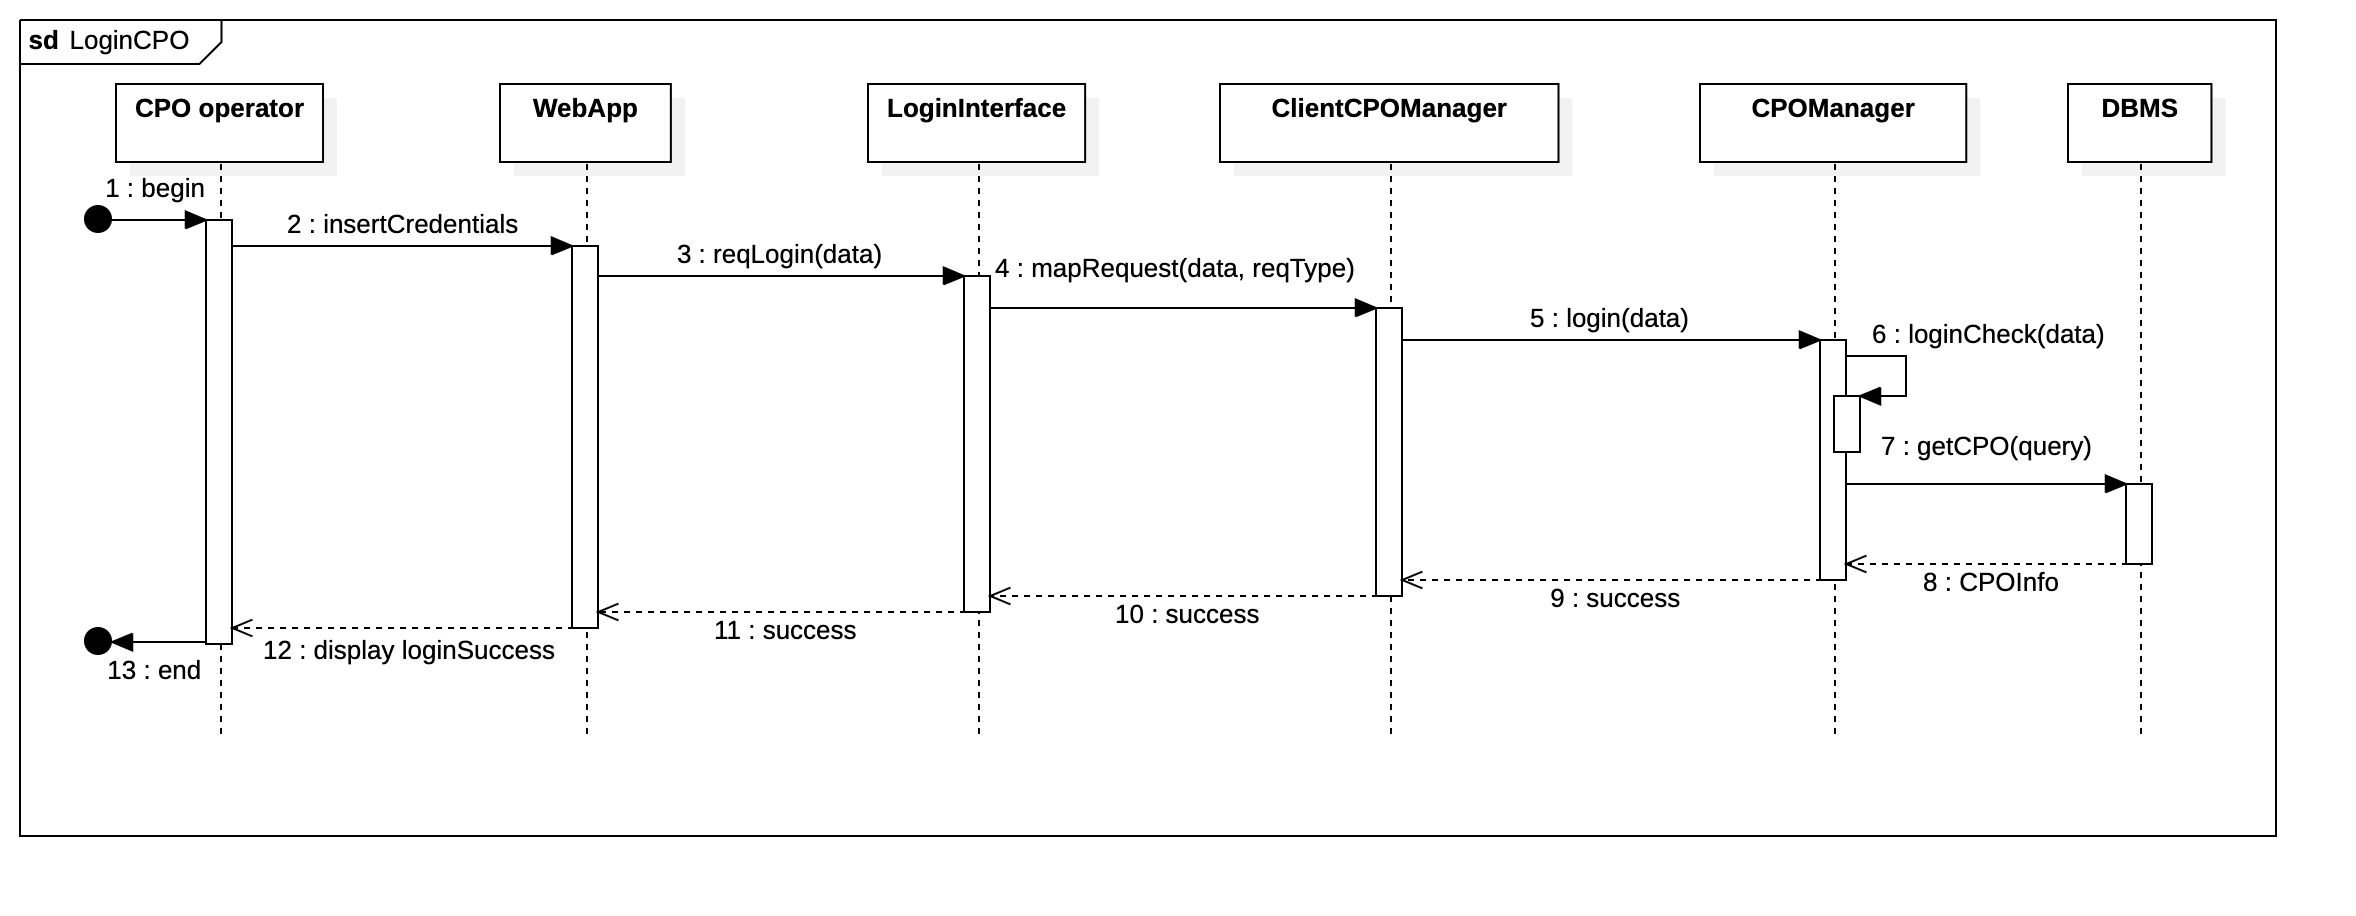
\includegraphics[width=\textwidth]{img/runtime/cpo_login}
    \end{center}
\end{figure}
The CPO operator inputs his login credentials and then the WebApp sends the request, through the CPOLoginInterface to the ClientCPOManager, which forwards them to the CPOManager that checks for their correctness and then interrogates the DBMS and searches for the credentials. If the returned value is null the ClientManager sends a specific error message and the login fails, otherwise a 200 response status code is sent to the WebApp.
\subsubsection{View CPO dashboard}
\begin{figure}[H]
    \begin{center}
        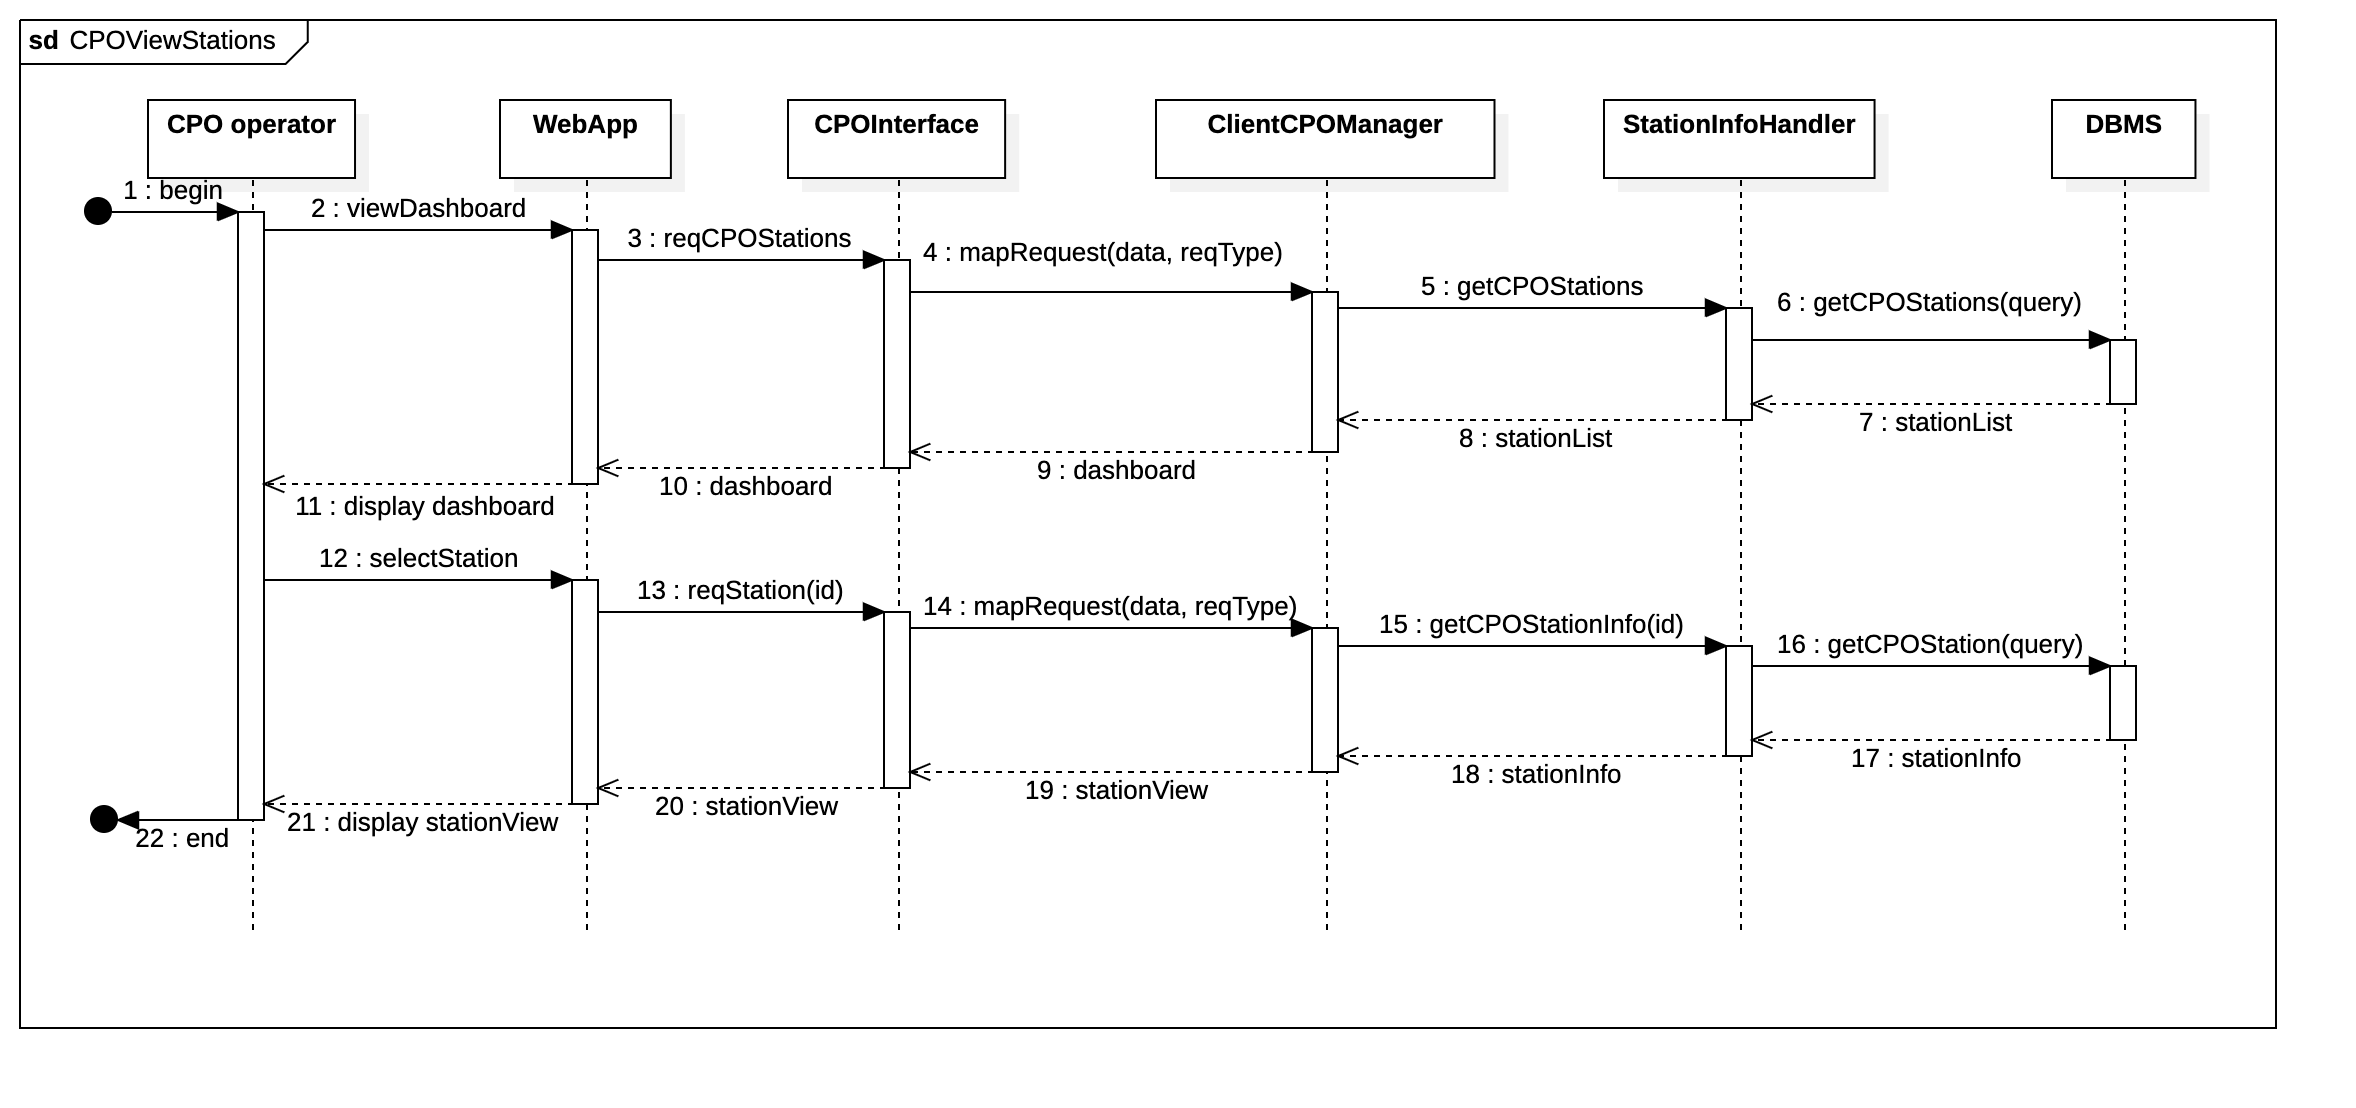
\includegraphics[width=\textwidth]{img/runtime/cpo_dashboard}
    \end{center}
\end{figure}
To access this view it is necessary to have performed the login before (\ref{cpo_login}). After the CPO operator login, the WebApp automatically request the dashboard where all the CPO's station are present. The WebApp contacts the ClientCPOManager through the CPOInterface. Then the StationInfoHandler is accessed, that in turn queries the DBMS to retrieve the list of charging stations associated with the CPO. The CPO main dashboard is then shown to the operator. If an operator wants to select the single station's dashboard, he can click the "modify" button that triggers the request from the WebApp to the StationInfoHandler, in the same way as before. The CPO operator can then view the station's current status and settings.
\subsubsection{Modify a station current charging price}
\begin{figure}[H]
    \begin{center}
        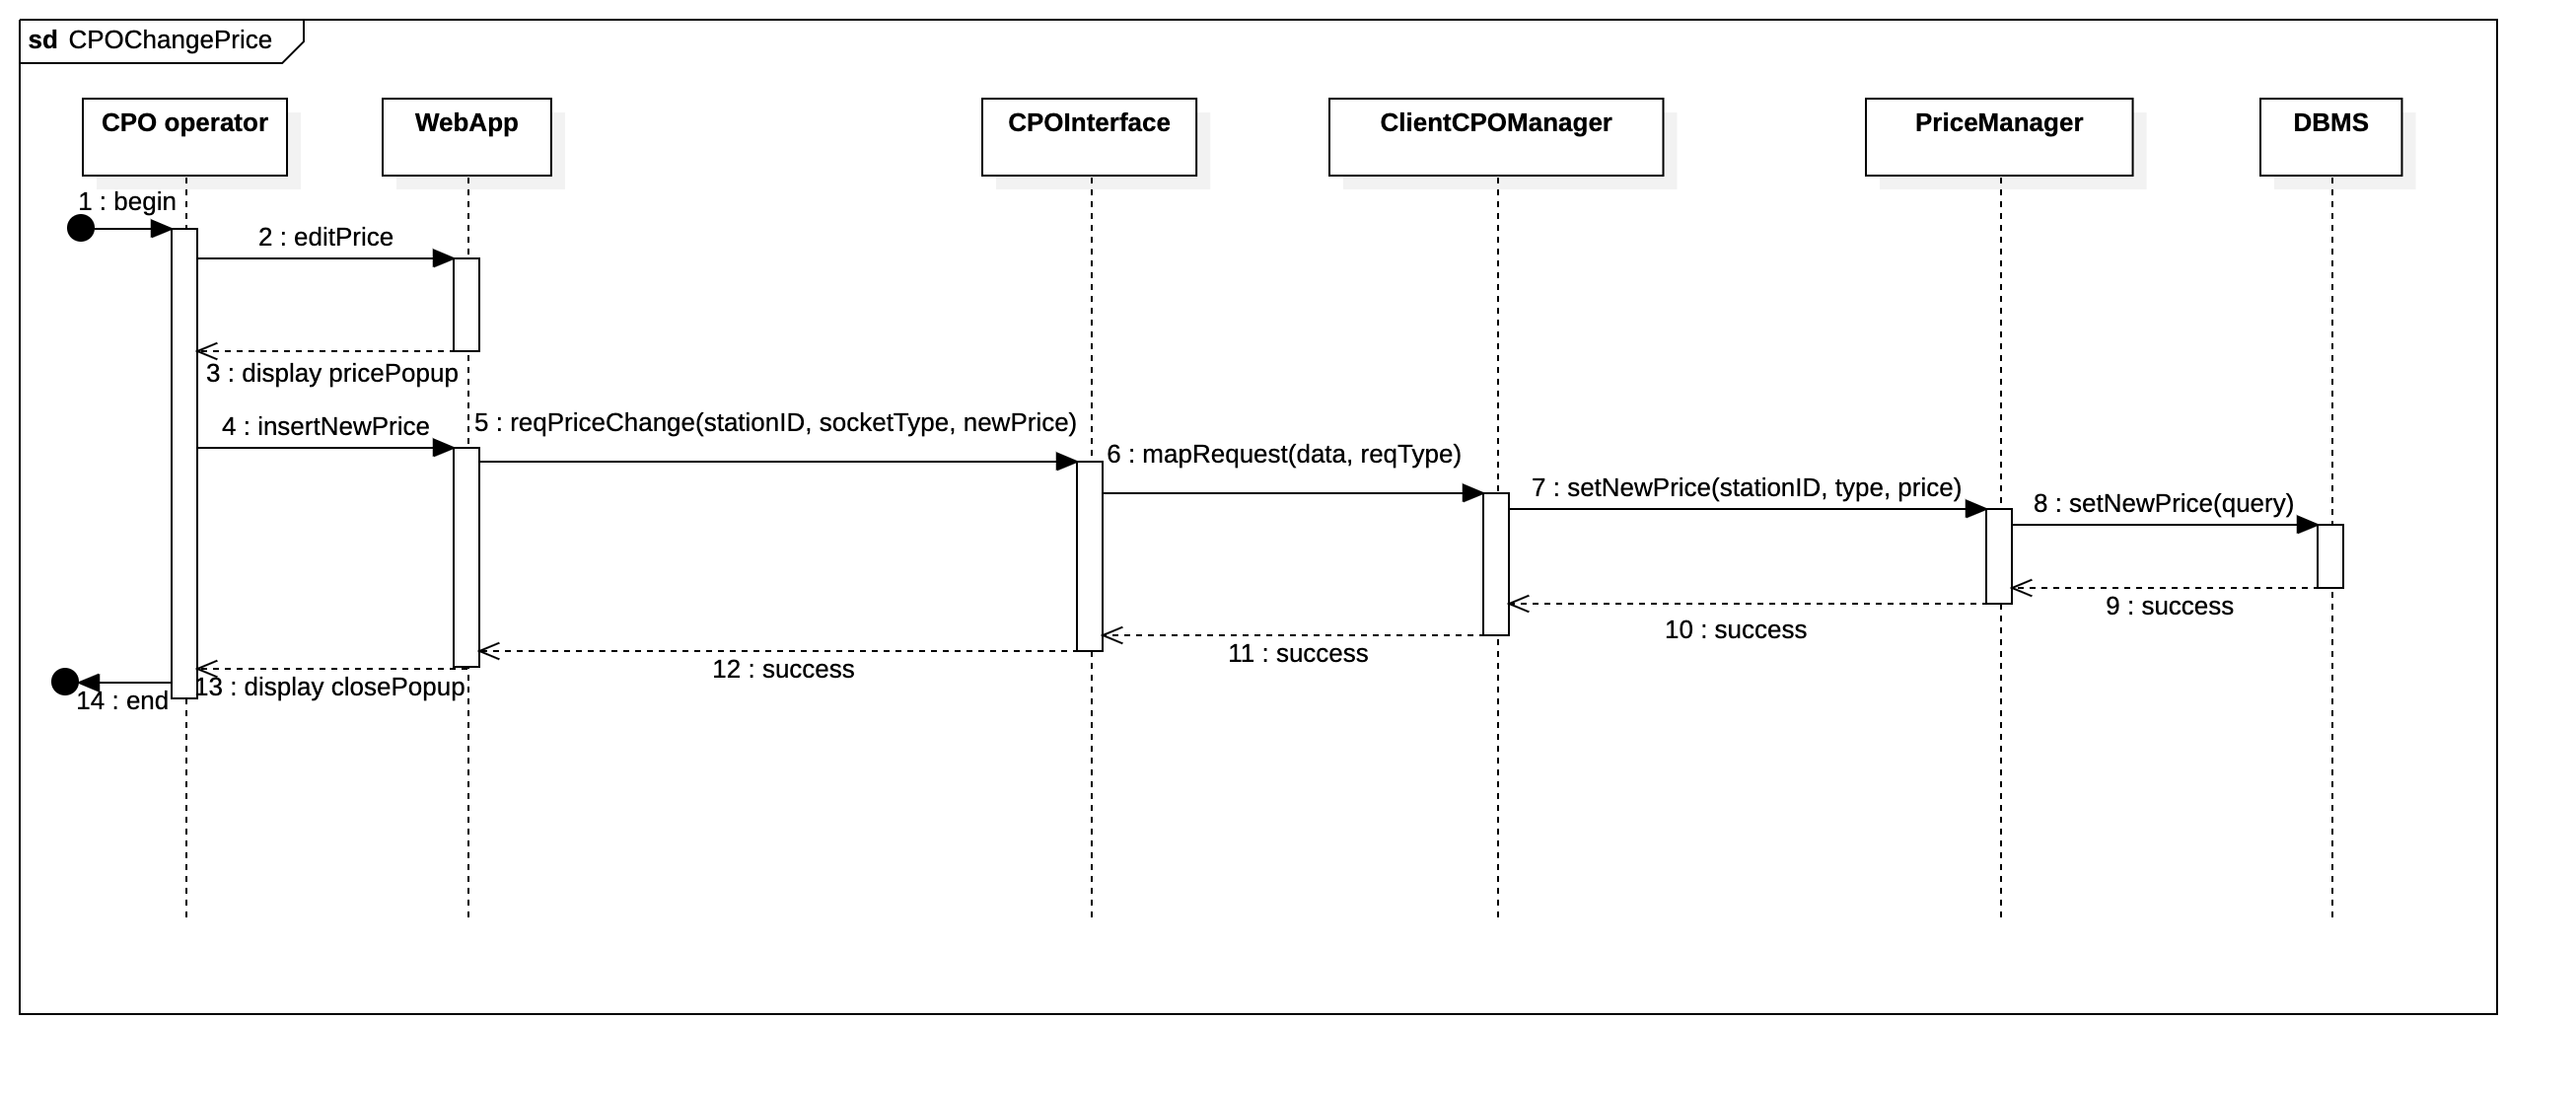
\includegraphics[width=\textwidth]{img/runtime/cpo_price}
    \end{center}
\end{figure}
To access this view it is necessary to have performed the login before (\ref{cpo_login}). The CPO operator must access the single station dashboard. In order to edit the station's current charging price, the "Update price" button must be selected. Then the WebApp will show a popup where the operator can enter the new price.
When a new price is entered, the WebApp contacts the ClientCPOManager through the CPOInterface, and finally the PriceManager is accessed. The PriceManager will store the station's new price in the CPMS' DBMS. The WebApp will be sent a 200 OK status code that will automatically close the popup.
\subsubsection{Modify a station current energy provider (DSO)}
\begin{figure}[H]
    \begin{center}
        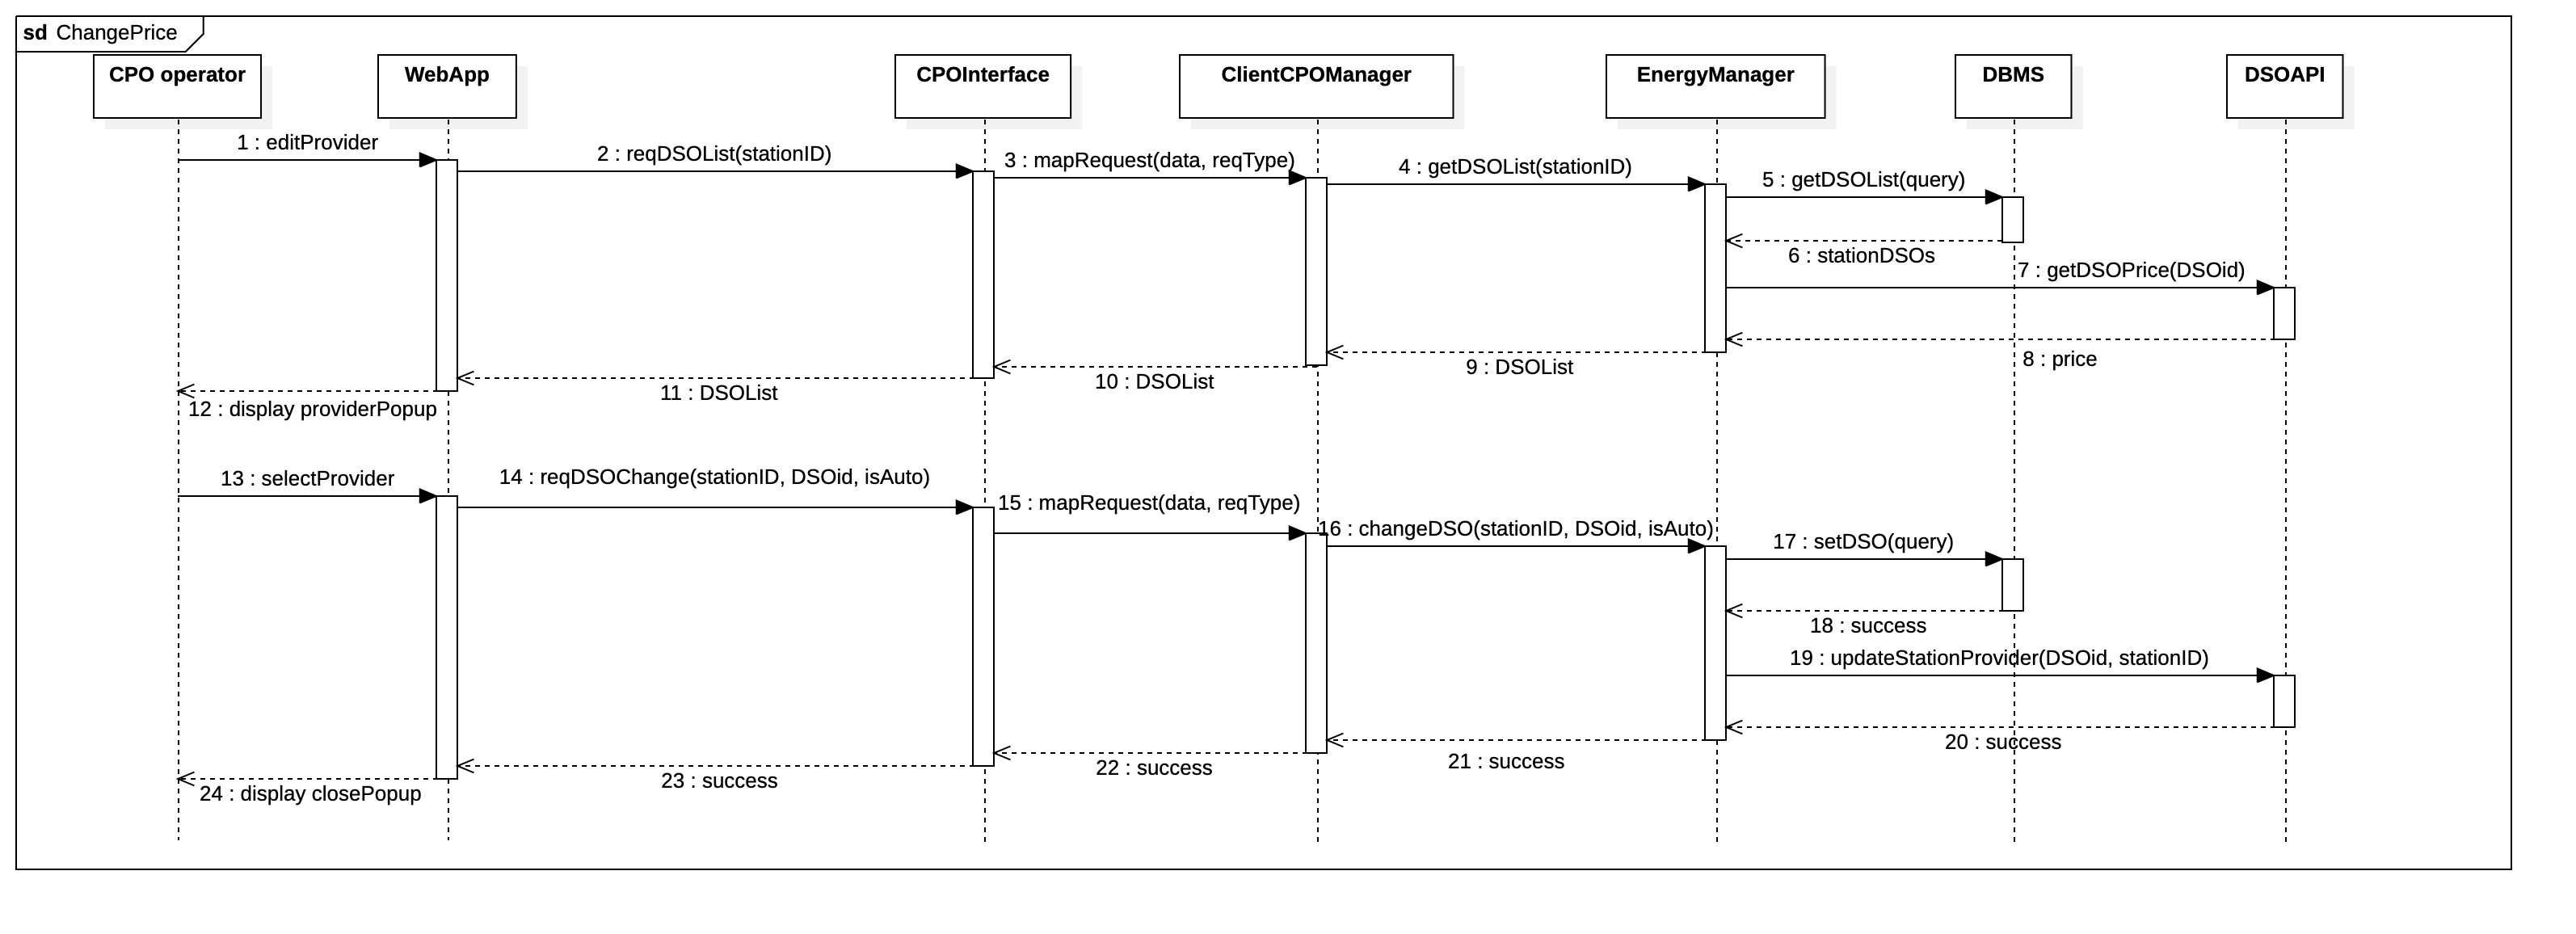
\includegraphics[width=\textwidth]{img/runtime/cpo_dso}
    \end{center}
\end{figure}
To access this view it is necessary to have performed the login before (\ref{cpo_login}). The CPO operator must access the single station dashboard. In order to edit the station's current energy provider (DSO), the "Update provider" button must be selected. Then the WebApp will contact the ClientCPOManager through the CPOInterface, and finally the EnergyManager is accessed. The EnergyManager will query the DBMS in order to retrieve the station's DSO list. The module will then query the external DSOAPI to get their current energy price. Then the DSO list will be sent to the WebApp, that will show a popup with all the available DSOs with their current prices.Finally, the operator can select either the automatic option or a manual DSO to acquire energy from. When a new option is selected, the WebApp contacts the EnergyManager again in the same way, but this time it updates the current station provider in the DBMS, and then it contacts the external DSOAPI to propagate the change.
The WebApp is returned a 200 OK status code that automatically closes the popup.
\subsubsection{Modify a station special offers}
\begin{figure}[H]
    \begin{center}
        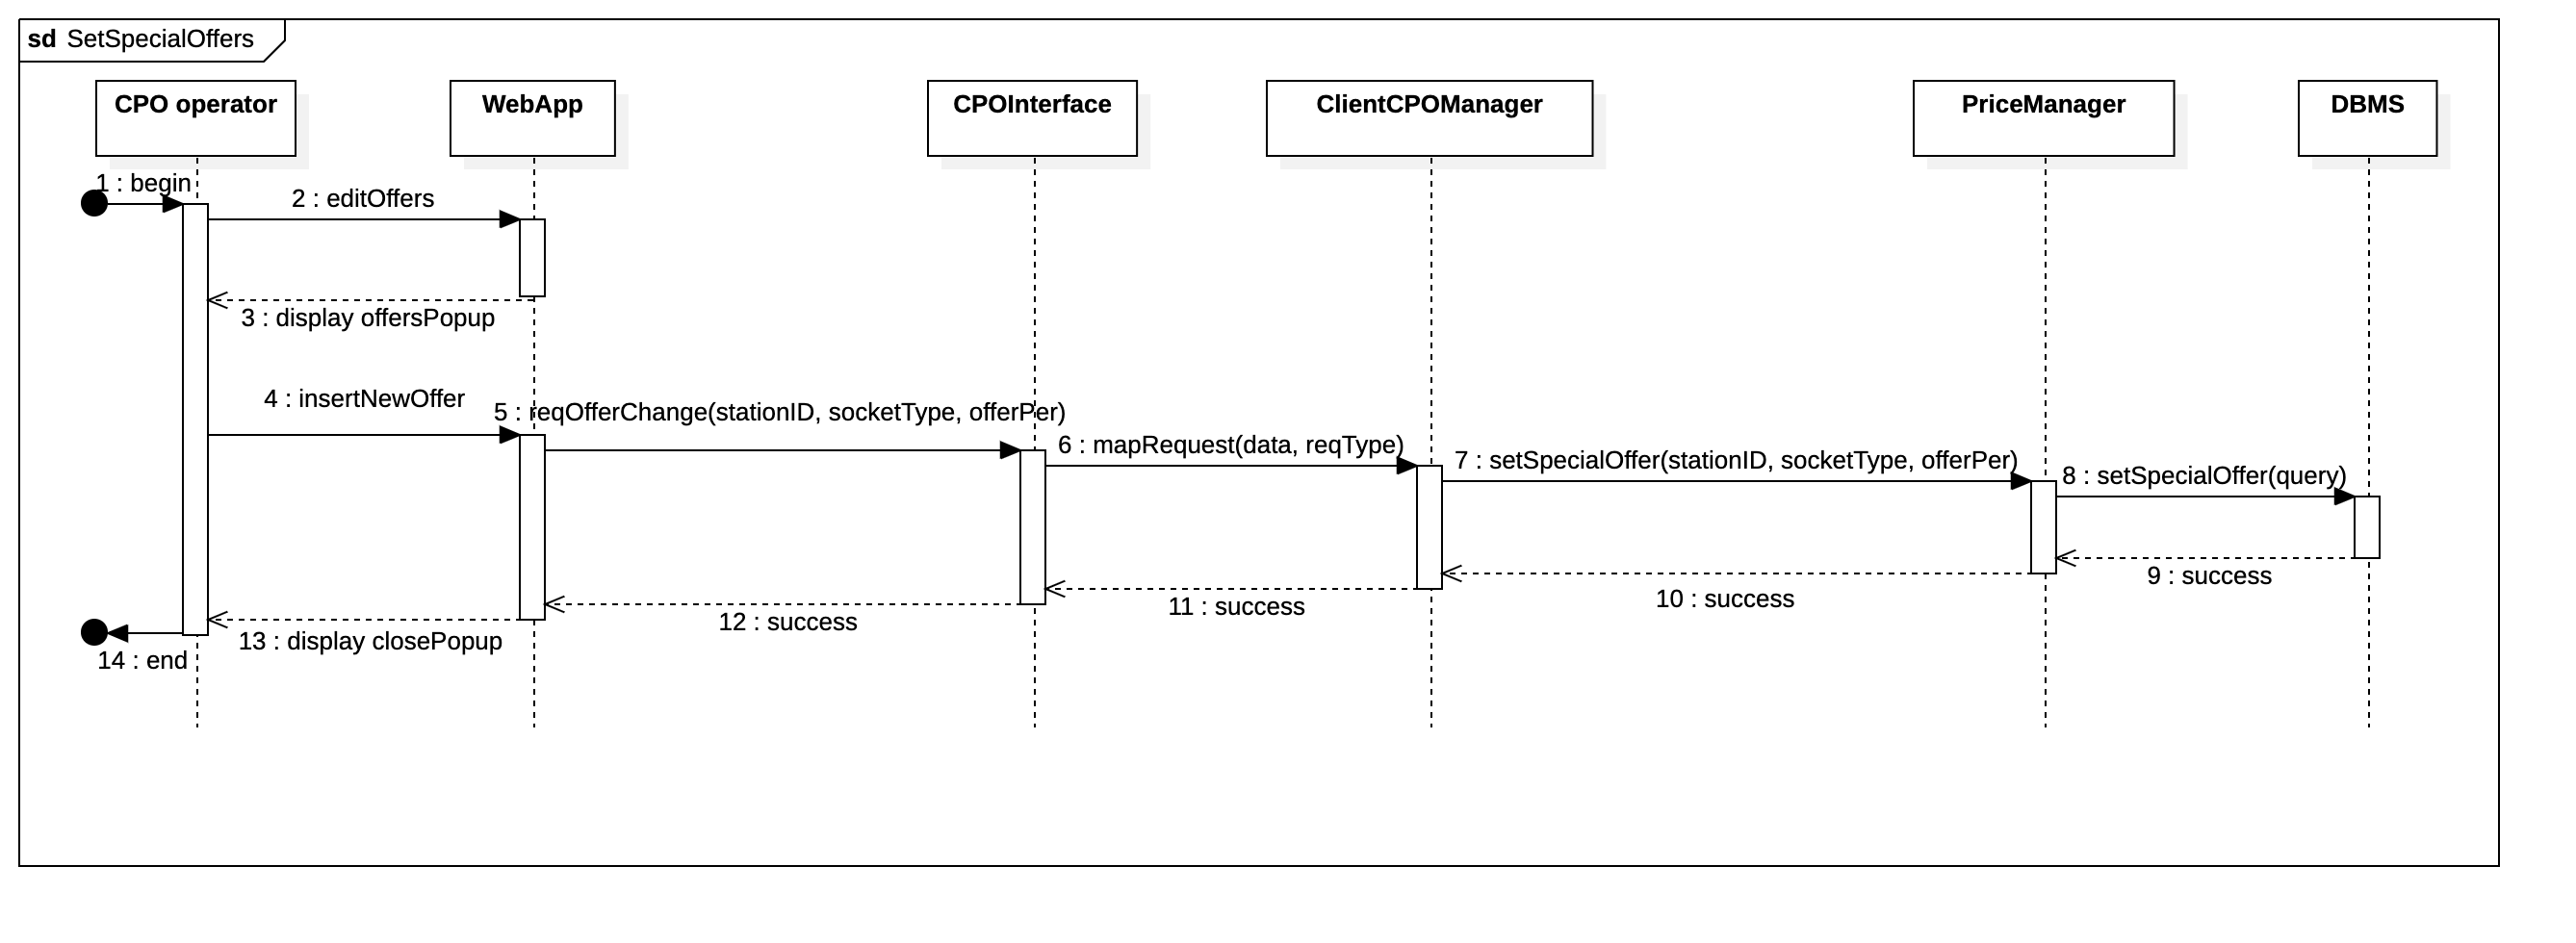
\includegraphics[width=\textwidth]{img/runtime/cpo_offers}
    \end{center}
\end{figure}
To access this view it is necessary to have performed the login before (\ref{cpo_login}). The CPO operator must access the single station dashboard. In order to edit the station's current special offers, the "Update special offer" button must be selected. Every special offer is bound to a type of charging socket. After the button is selected, the WebApp will show a popup where the operator can enter the new special offer for the type of socket.
When a new offer is entered, the WebApp contacts the ClientCPOManager through the CPOInterface, and finally the PriceManager is accessed. The PriceManager will store the station's new offer in the CPMS' DBMS. The WebApp will be sent a 200 OK status code that will automatically close the popup.
\subsubsection{Modify a station battery policy}
\begin{figure}[H]
    \begin{center}
        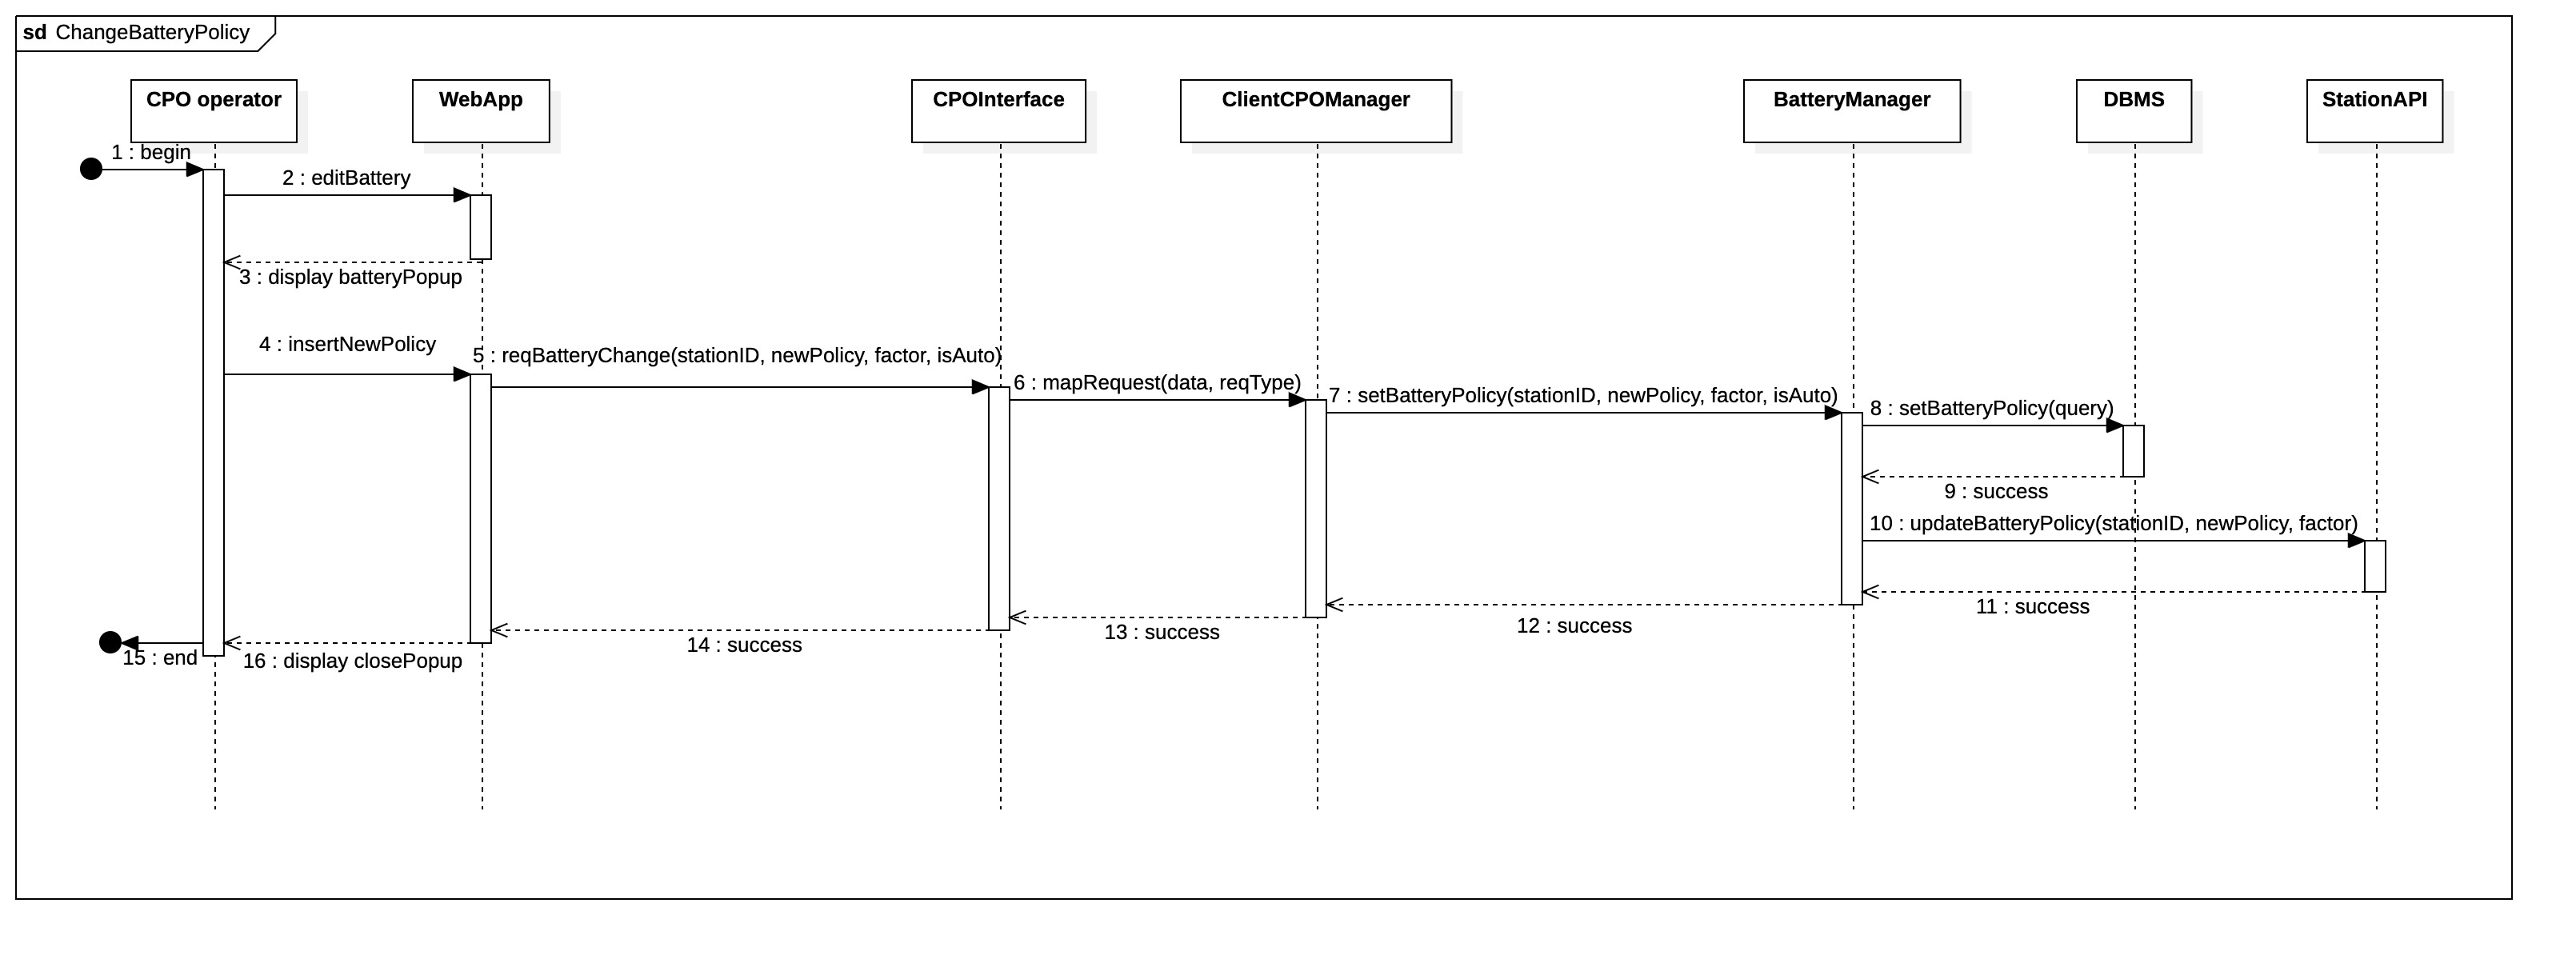
\includegraphics[width=\textwidth]{img/runtime/cpo_battery}
    \end{center}
\end{figure}
To access this view it is necessary to have performed the login before (\ref{cpo_login}). The CPO operator must access the single station dashboard. Another requirement lies in the fact that the station has to have a battery installed. In order to edit the station's current battery policy, the "Update battery policy" button must be selected. After the button is selected, the WebApp will show a popup where the operator can enter the new battery policy of the station. Finally, the operator can select either the automatic option or a manual battery policy. When a new option is selected, the WebApp contacts the ClientCPOManager through the CPOInterface. The next step is to access the BatteryManger that will update the battery policy on the DBMS and then apply the policy to the station by contacting the external StationAPI. The WebApp is returned a 200 OK status code that automatically closes the popup.
\subsection{Component interface}

\begin{figure}[H]
    \begin{center}
        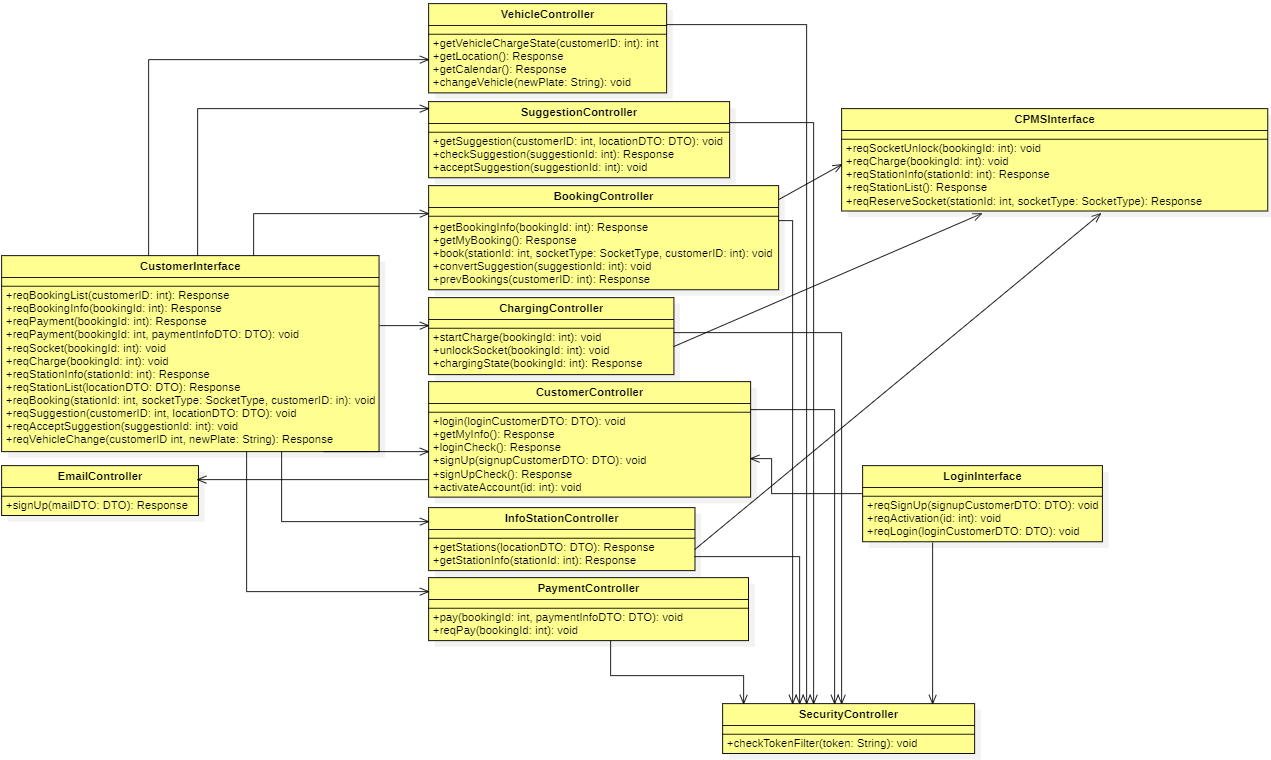
\includegraphics[width=\textwidth]{img/ComponentInterface1.PNG}
        \caption{Component Interface 1}\label{component_interface1}
    \end{center}
\end{figure}

\begin{figure}[H]
    \begin{center}
        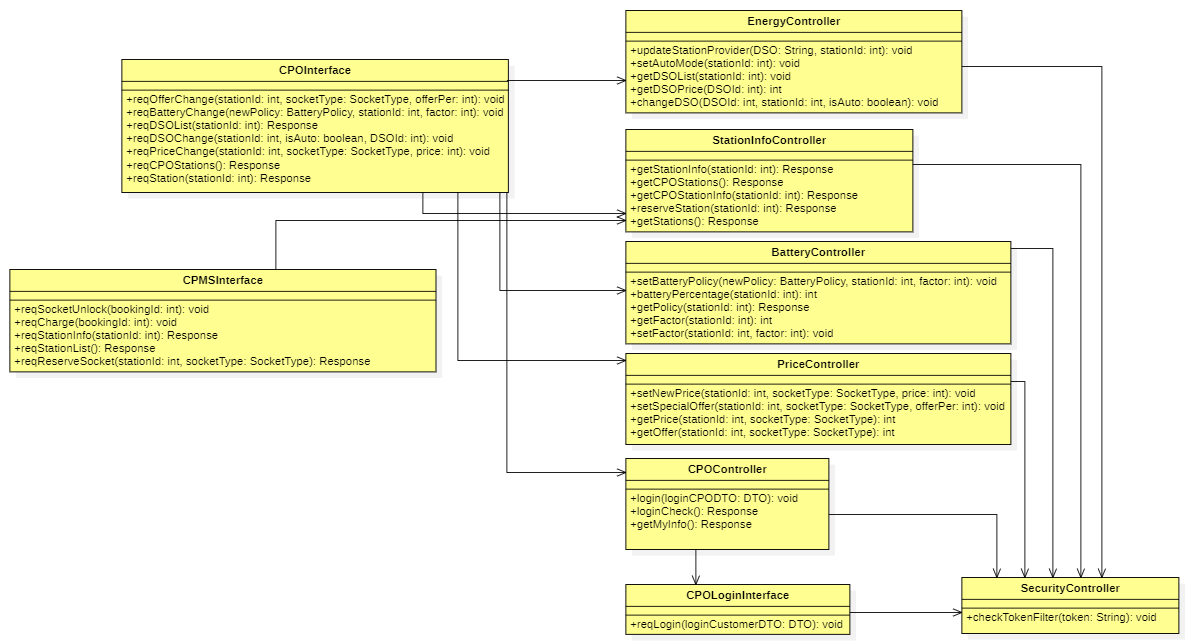
\includegraphics[width=\textwidth]{img/ComponentInterface2.PNG}
        \caption{Component Interface 2}\label{component_interface2}
    \end{center}
\end{figure}

eMSP interfaces description:
\begin{itemize}
    \item \textbf{CustomerInterface}: this is the main interface to exchange data between the mobile-application and the eMSP.
    \item \textbf{LoginInterface}: this interface is used to handle the login, sign-up, and account activation of the customer. It's used to comunicate between the mobile-app and the eMSP.
    \item \textbf{SecurityController}: eMSP's internal interface, used to manage the authorization of the user operations (operations of the CustomerInterface and LoginInterface). It's used by each component to validate the request token.
    \item \textbf{VehicleController}: eMSP's internal interface, used to handle the request and data exchanged with the VehicleApi. It offers all the methods related with the user-vehicle.
    \item \textbf{SuggestionController}: eMSP's internal interface, used to comunicate with the SuggestionHandler, it exposes methods to find candidate suggestions, to accept suggestions.
    \item \textbf{BookingController}: eMSP's internal interface, used to manage customer's bookings. It exposes methods to create a new booking, get info about a booking, get all booking (olds and current). 
    \item \textbf{ChargingController}: eMSP's internal interface, used to manage the vehicle charging process. For example the startCharge method is used to start a booked charge.
    \item \textbf{CustomerController}: eMSP's internal interface, it is linked with the LoginInterface. It is used to internally perform login-signup operations.
    \item  \textbf{InfoStationController}: eMSP's internal interface, it is used to retrive station informations. The method getStationInfo for example returns all the info about a station: socket availability, charging price
    \item \textbf{PaymentController}: eMSP's internal interface, it is used to manage the payment phase. The reqPay method is used to send a payment request. The pay method is used to communicate the payment informations and pay.
\end{itemize}

CPMS interfaces description:
\begin{itemize}
    \item \textbf{CPMSInterface}: this is the main interface to exchange data between the eMSP and the CPMS. It can be retrived a list of stations, or info about a single station. It can be requested to unlock a socket or request a reservation for a booking.
    \item \textbf{CPOInterface}: this is the main interface to exchange data between the CPMS and the CPO-WebServer. It expose all the functionalities to manage a station, for example to set special offers, set charging price...
    \item \textbf{CPOLoginInterface}: this is the interface to handle CPO's login. It is an interface between the CPMS and the CPO-WebServer.
    \item \textbf{EnergyController}: CPMS's internal interface, it is used to manage the DSO providers. To retrive the DSO prices. To set the acquisition of energy to automatic mode.
    \item \textbf{StationInfoController}: CPMS's internal interface, mainly used to retrive stations' information. It is also used to make a reservation for a socket.
    \item \textbf{BatteryController}: CPMS's internal interface, it is used to control the station's batteries. It exposes methods to set the battery policy (mantain, charge or discharge), set discharging factor, or retrive information.
    \item \textbf{PriceController}: CPMS's internal interface, it is used to set and retrive charging prices and to set special offers.
    \item \textbf{CPOController}: CPMS's internal interface, it is linked with the CPOLoginInterface. It is used to internally perform login operations.
    \item \textbf{SecurityController}: CPMS's internal interface, used to manage the authorization of the user operations (operations of the CustomerInterface and LoginInterface). It's used by each component to validate the request token.
    
\end{itemize}

\subsection{Selected architectural styles and patterns}

\subsubsection{Four-tiered architecture}
We chose this architecture for many reasons:
\begin{itemize}
    \item \textbf{Flexibility:} Once the interfaces of the S2B are defined, then the interior logic is independent from outside. Single components can therefore be implemented in parallel. And can be modified without affecting the system.
    \item \textbf{Scalability:} An application divided on several tiers guarantees that the approach of scaling the architecture is adopted only for the most critical components. The result obtained maximizes the performance but also minimizes the costs.
    \item \textbf{Load Distribution:} the presence of several application servers, preceded by a load balancer, guarantees an acceptable division of requests. Otherwise, the presence of a single node means that node can become over-requested, sending the entire system down.
\end{itemize}

\subsubsection{RESTful Architecture}
\label{REST}
The restful application will be adopted both on web and mobile side. This architecture is based on the stateless principle, in which the server does not contain any information about the state of client, that is managed directly on client side.

An useful property of this architecture is the \textit{code on demand} one, which permits sending some code snippets from the server to the client, and then make the client executing them locally (usually in the web browser). This behavior guarantees less computational load on the server and also a dynamic attitude of the service.

The application is then intended to be developed through \textit{client side scripting}, which means that all requests and update of the page are made on client side. This behavior also improves the user experience, and prevent refreshing the page each time an action is made.

\subsubsection{Model View Controller (MVC)}
Model--View--Controller (usually known as MVC) is a software design pattern commonly used for developing user interfaces that divides the related program logic into three interconnected elements. This is done to separate internal representations of information from the ways information is presented to and accepted from the user.

These three components are:
\begin{itemize}
    \item \textbf{Model:} the central component of the pattern. It is the application's dynamic data structure, independent of the user interface. It directly manages the data, logic and rules of the application.
    \item \textbf{View:} any representation of information such as a chart, diagram or table. Multiple views of the same information are possible, such as a bar chart for management and a tabular view for accountants.
    \item \textbf{Controller:} accepts input and converts it to commands for the model or view.
\end{itemize}

\subsection{Other design decisions}
\subsubsection{Scale-Out}
This method consists of cloning the nodes in which we expect to have a bottleneck in order to increase the general system scalability.

This choice leads to a higher deployment effort but also to a lower hardware upgrade cost when the limits are reached. In conclusion, the scale-out is a preferable road.

Once split, the system requires a load balancer in order to correctly redirects the incoming requests to the node with the lowest workload.

\subsubsection{Thin and thick client and fat server}
The thin client will be the web application.\\
This architecture consists of keeping as low information as possible on client side. It means that the business logic resides only on server side.\\
The minimum requirement of this choice is a stable connection between the parts; otherwise the application would not work as expected.\\
Of course, the main advantage of choosing this implementation style is that the client machine is not required to have an high computational power.

Instead, in the case of mobile application, the best choice is to save useful information on a local database, in order to avoid continuous requests to the server (less computational load) and also to keep information even when the Internet connection is not available. 
In this second case it is said to be a thick client.

\subsubsection{Automatic-DSO-Energy-Source selection - Algorithm}
When the CPMS system has the automatic DSO feature active, an algorithm to automatically choose a DSO is used. The choice of the energy source is based on the minimum price available (with the assumption that energy availability is not an issue). The DSO that offers the minimum price is choosen. Every 30min a scan for the minimum price DSO is performed and if a better DSO is find, the energy source is changed.


\subsubsection{Automatic-Battery-Mode selection - Algorithm}
When the CPMS system has the automatic battery mode active, an algorithm to automatically managed the battery operation mode  (Discharge, Mantain, Recharge) is used. When the battery is in discharge mode, it means that the battery is discharging and the energy is flowing from the battery to the vehicles, when the battery is in mantain mode it is not used. The automatic battery mode uses the policy in figure \ref{battery_policy}. Once activated the automatic mode the battery state is mantain. Every time the battery state of charge (SoC) is less than 20 \% it goes to the recharge state.
The transition between mantain and discharge states are based on the station socket occupation: if there are many customers (>50 \% of sockets occupied) the battery is set to discharge state, if insted the occupation becomes lower than 40 \% (debouncing factor) the battery is deactivated.

\begin{center}
    \begin{figure}[H]
        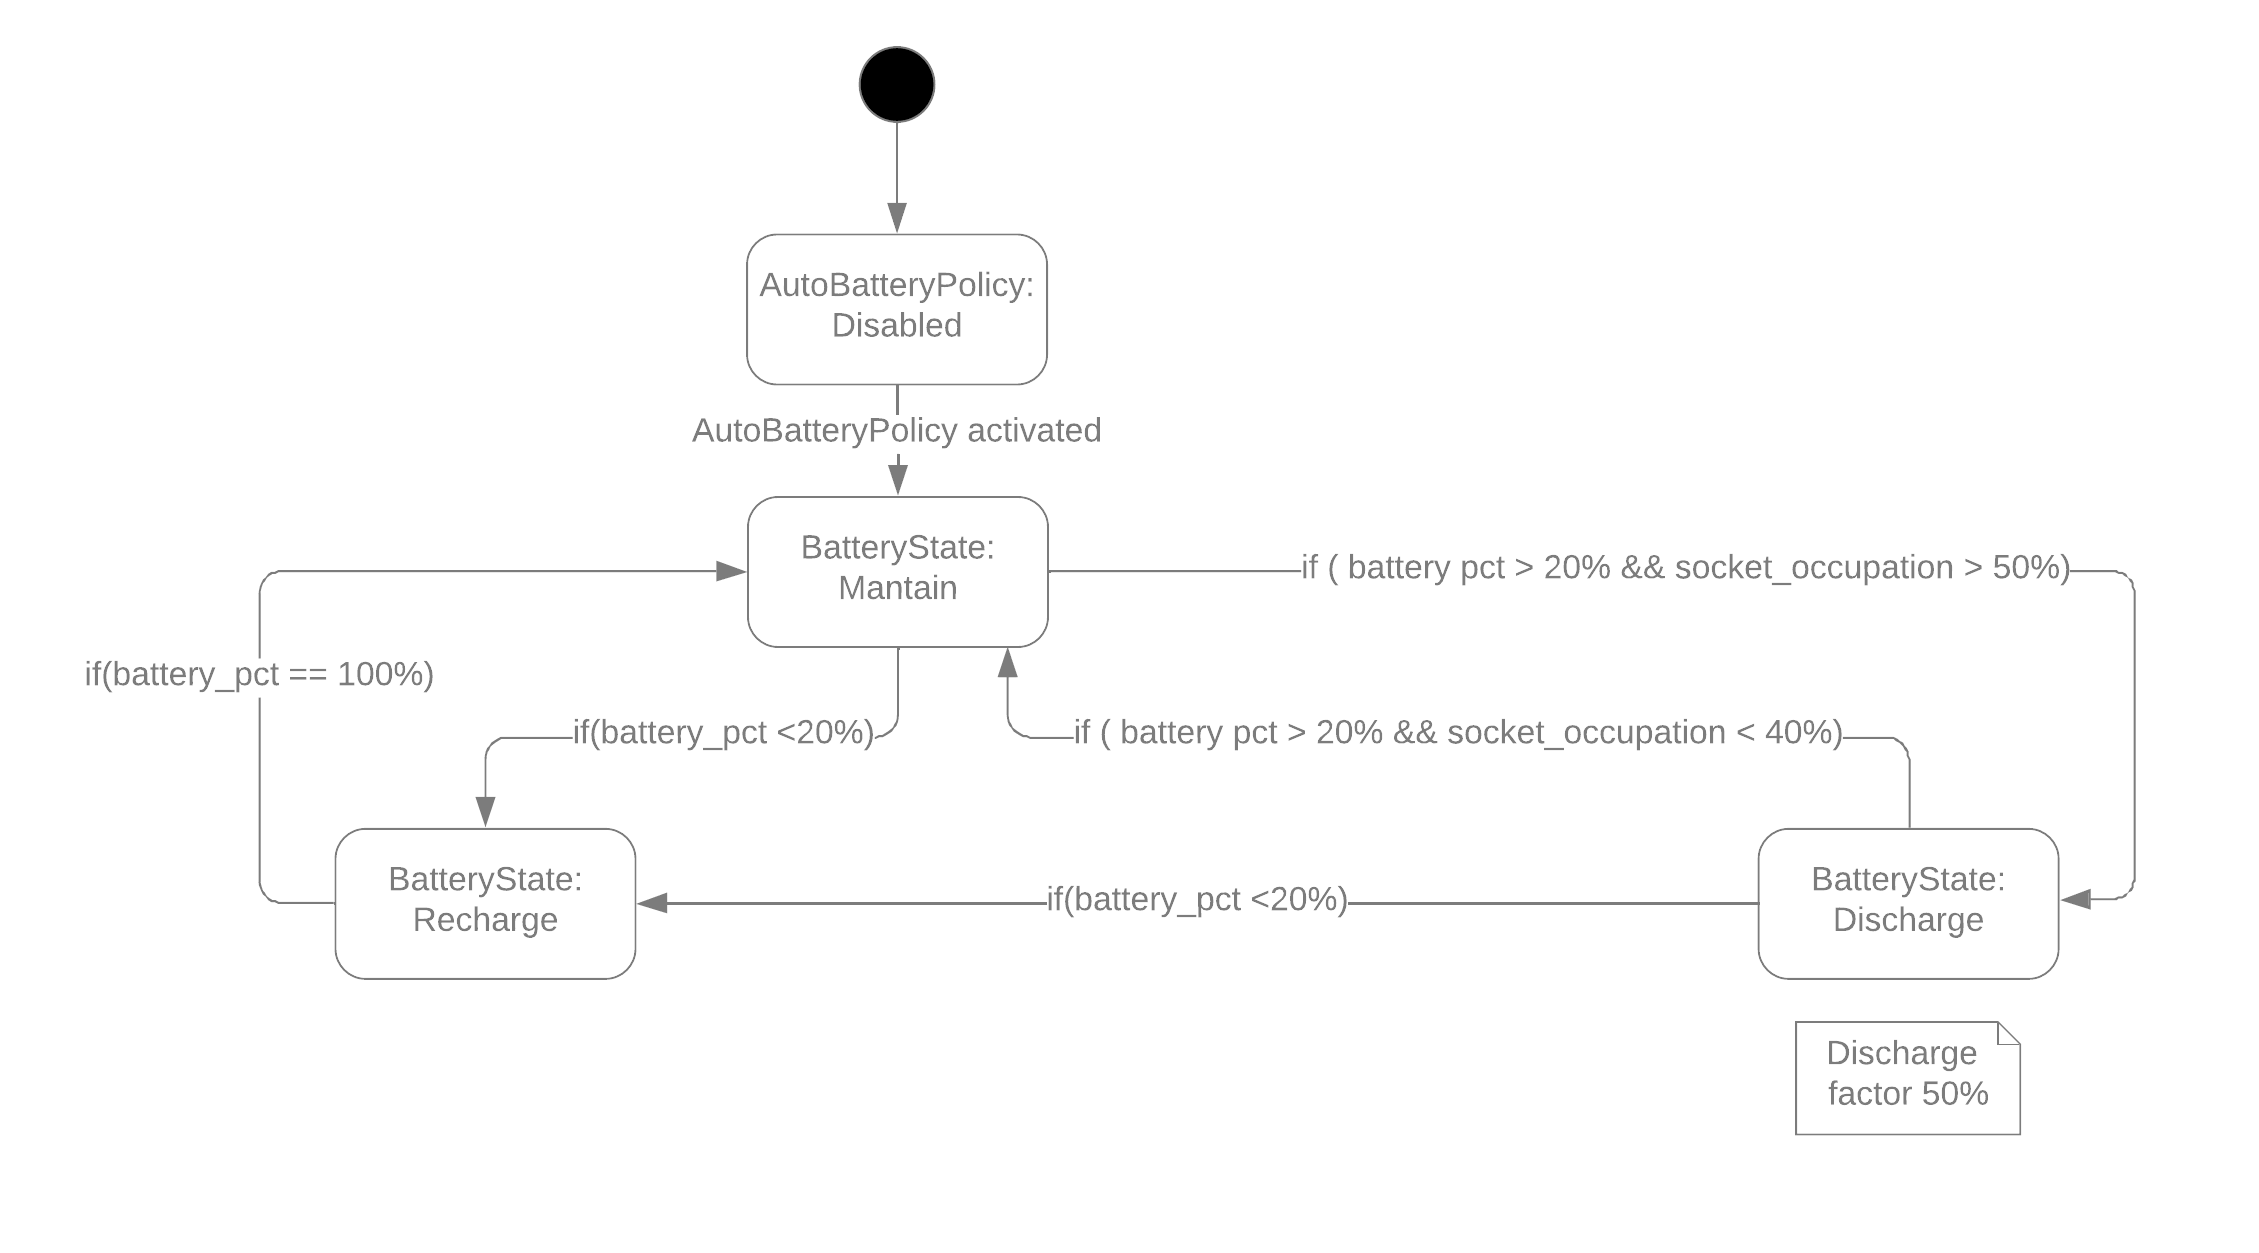
\includegraphics[width=\textwidth]{./img/battery_policy.png}
        \caption{Automatic battery policy state machine}
        \label{battery_policy}
    \end{figure}
\end{center}

\subsubsection{Send-suggestions - Algorithm}
The eMSP sends booking suggestions to the customer's mobile-app. Suggestions are based on customer position, car's SoC, calendar. A basic algorithm will send suggestions only when the customer has at least the next 3 hours free, the battery SoC must be under the 60\%. The application will not "spam" noification, so a debouncing time of 2h is set between one suggestion and another. The suggested charging station is simply the nearest to the customer's location.